\documentclass[%
pdf,
%nocolorBG,
colorBG,
slideColor,
%slideBW,
%draft,
%frames
%azure
%contemporain
%nuancegris
%troispoints
%lignesbleues
%darkblue
%alienglow
%autumn
]{prosper}
\usepackage{pifont, amsmath, multicol}
%\usepackage{floatflt, wrapfig,subfigure}
%\usepackage{wrapfig}
%\usepackage{floatflt}
\usepackage{color}
\usepackage{epsfig}
\usepackage{pifont}
\usepackage[T1]{fontenc}
\usepackage[latin1]{inputenc}
\def\QuotS#1#2{\leavevmode\kern-.0em\raise.2ex\hbox{$#1$}\kern-.1em/\kern-.1em\lower.25ex\hbox{$#2$}}


%\usepackage[francais]{babel}
%\def«{\og\ignorespaces}%
%\def»{{\fg}}%
\newcommand{\spacer}{\rule[-3mm]{0mm}{8mm}}
\newtheorem{theorem}{Theorem}
\newtheorem{definition}[theorem]{Definition}

\newcommand{\RR}{\ensuremath{\mathbb{R}}}
\newcommand{\NN}{\ensuremath{\mathbb{N}}}
\newcommand{\QQ}{\ensuremath{\mathbb{Q}}}
\newcommand{\CC}{\ensuremath{\mathbb{C}}}
\newcommand{\ZZ}{\ensuremath{\mathbb{Z}}}
\newcommand{\TT}{\ensuremath{\mathbb{T}}}

\def\QuotS#1#2{\leavevmode\kern-.0em\raise.2ex\hbox{$#1$}\kern-.1em/\kern-.1em\lower.25ex\hbox{$#2$}}


\title{\Huge \textcolor{blue}{Zigzags and central circuits for $3$- or $4$-valent plane graphs}}
%\textcolor{blue}{and generalizations}}

\author{
\begin{multicols}{2}
\textcolor{red}{\Large Michel Deza}\\[2mm]
\textcolor{black}{\large ENS/CNRS, Paris and ISM, Tokyo}\\[2mm]
\textcolor{red}{\Large Mathieu Dutour}\\[2mm]
%\textcolor{red}{\large ENS/CNRS, Paris and Hebrew University, Jerusalem}\\[2mm]
\textcolor{black}{\large Ruder Boskovic Institute, Zagreb}\\[2mm]
\textcolor{red}{\Large Mikhail Shtogrin}\\[2mm]
\textcolor{black}{\large Steklov Institute, Moscow}\\[2mm]
\textcolor{red}{\Large Patrick Fowler}\\[2mm]
\textcolor{black}{\large Exeter University}
\end{multicols}
\begin{center}
\textcolor{red}{\Large Frank Vallentin}\\[2mm]
\textcolor{black}{\large Hebrew University, Jerusalem}
\end{center}


}


\slideCaption{}

\date{}



\begin{document}
\maketitle




\begin{slide}{}
\begin{center}
{\Huge 
\begin{tabular*}{9cm}{c}
\\[-0.5cm]
\textcolor{blue}{I. }\textcolor{red}{$k$-valent}\\
\textcolor{red}{two-faced polyhedra}
\end{tabular*}
}
\end{center}
\end{slide}




\begin{slide}{Polyhedra and planar graphs}
\vspace{-2mm}

A graph is called \textcolor{red}{$k$-connected} if after removing any set of $k-1$ vertices it remains connected.

\vspace{2mm}

The \textcolor{red}{skeleton} of a polytope $P$ is the graph $G(P)$ formed by its vertices, with two vertices adjacent if they generate a face of $P$.
%
%\vspace{3mm}

{\em {\bf Theorem} (Steinitz)

(i) A graph $G$ is the skeleton of a $3$-polytope if and only if it is planar and $3$-connected.

(ii) $P$ and $P'$ are in the same \textcolor{red}{combinatorial type} if and only if $G(P)$ is isomorphic to $G(P')$.
}

\vspace{3mm}

The \textcolor{red}{dual} graph $G^*$ of a plane graph $G$ is the plane graph formed by the faces of $G$, with two faces adjacent if they share an edge.




\end{slide}



\overlays{2}{
\begin{slide}{Example}
\onlySlide*{1}{
\begin{center}
\begin{minipage}{5cm}
\centering
\epsfxsize=2.5cm
\epsfig{figure=CanadaPicture/CubePlanar1.eps, height=3cm}\par
The regular cube
\end{minipage}
\begin{minipage}{5cm}
\centering
\epsfig{figure=CanadaPicture/CubePlanar2.eps, height=3cm}\par
its planar graph
\end{minipage}
\end{center}
}
\onlySlide*{2}{
\begin{center}
\begin{minipage}{5cm}
\centering
\epsfxsize=2.5cm
\epsfig{figure=CanadaPicture/CubePlanar3.eps, height=3cm}\par
A perturbed cube
\end{minipage}
\begin{minipage}{5cm}
\centering
\epsfig{figure=CanadaPicture/CubePlanar2.eps, height=3cm}\par
its planar graph
\end{minipage}
\end{center}
A $3$-polytope is usually  represented by the Schlegel diagram of its skeleton, the program used for this is \textcolor{blue}{CaGe} by \textcolor{blue}{G. Brinkmann}, \textcolor{blue}{O. Delgado}, \textcolor{blue}{A. Dress} and \textcolor{blue}{T. Harmuth}.
}

\end{slide}
}





%A polyhedron is called \textcolor{red}{simple} if all its vertices are $3$-valent.
%\vspace{3mm}
\begin{slide}{$k$-valent two-faced polyhedra}
The Euler formula for plane graphs \textcolor{red}{$V-E+F=2$},\\
take the following form for $k$-valent graphs:
\begin{equation*}
\begin{array}{rcl}
12=\sum_{i} (6-i) p_i&\mbox{~if~}&\textcolor{red}{k=3}\\
\mbox{~~and~~}8=\sum_{i} (4-i) p_i&\mbox{~if~}&\textcolor{red}{k=4}
\end{array}
\end{equation*}
With $p_i$ the number of faces of \textcolor{red}{gonality} $i$.

A $k$-valent plane graph is called \textcolor{red}{two-faced} if the gonality of its faces has only two possible values $a$ and $b$.

\begin{itemize}
\item $3$-valent plane graphs with $n$ vertices and faces of gonality $q$ and $6$ (\textcolor{red}{classes $q_n$}),
\item $4$-valent plane graphs with $n$ vertices and faces of gonality $3$ or $4$ (\textcolor{red}{octahedrites}).
\end{itemize}

%\begin{center}
%$a$ and $b$, where $3\leq a< b\leq 6$ or $4$.
%\end{center}%\begin{center}
%there are $3$ cases: $3_n$, $4_n$, $5_n$.
%\end{center}
\end{slide}



\begin{slide}{Examples}
\begin{center}
\begin{minipage}{5cm}
\centering
\epsfxsize=2.5cm
\epsfig{figure=OCT2picture/8-hedrite12_2.eps, height=3cm}\par
An octahedrite
\end{minipage}
\begin{minipage}{5cm}
\centering
\epsfig{figure=ZIG2picture/First3nD2.sec.eps, height=3cm}\par
A $3_{24}$ plane graph
\end{minipage}
\begin{minipage}{5cm}
\centering
\epsfig{figure=CanadaPicture/Graph26_2Nude.eps, height=3cm}\par
A $4_{26}$ plane graph
\end{minipage}
\begin{minipage}{5cm}
\centering
\epsfig{figure=PictureAppli/F4sec.eps, height=3cm}\par
A $5_{28}$ plane graph
\end{minipage}


\end{center}
\end{slide}











\begin{slide}{Classes and their generation}
\vspace{-2mm}
{\tiny
\begin{center}
\begin{tabular}{||c|c||c|c|c|c||}
\hline
\hline
$k$ & $(a,b)$ & Polyhedra & Exist if and only if & $p_a$ & $n$\\ \hline\hline
$3$ & $(3,6)$ & $3_{n}$ & $\frac{p_{6}}{2} \in N-\{1\}$ & $p_3=4$ &$4+2p_6$\\  \hline
$3$ & $(4,6)$ & $4_{n}$ & $p_{6} \in N-\{1\}$ & $p_4=6$ &$8+2p_6$\\ \hline
$3$ & $(5,6)$ & $5_{n}$ (\textcolor{red}{fullerenes}) & $p_6\in N-\{1\}$& $p_5=12$ &$20+2p_6$\\ \hline\hline
$4$ & $(3,4)$ & \textcolor{red}{octahedrite} & $p_{4} \in N-\{1\}$ & $p_3=8$ &$6+p_4$\\ \hline\hline
%$(4,5)$ & 4 dual deltahedra & $p_5=2,3,4,5$ &$p_4=5,4,3,2$&$n=10,12,14,16$\\ \hline
%$(3,5)$ & D\"urer's Octahedron & $p_5=6$ &$p_3=2$ &$n=12$\\ \hline
%$(3,4)$ & Prism${}_{3}$ & $p_4=3$ & $p_3=2$ & $n=6$\\ 
\end{tabular}
\end{center}
}
\begin{center}
Generation programs
\end{center}

\begin{itemize}
\item \textcolor{red}{$3$-valent:} \textcolor{blue}{CPF} for two-faced maps on the sphere by \textcolor{blue}{T. Harmuth}\\
\textcolor{white}{$3$-valent:} \textcolor{blue}{CGF} for two-faced maps on surfaces of genus $g$ by \textcolor{blue}{T. Harmuth}
\item \textcolor{red}{$4$-valent:} \textcolor{blue}{ENU} by \textcolor{blue}{T. Heidemeier}
\item \textcolor{red}{General:} \textcolor{blue}{plantri} by \textcolor{blue}{G. Brinkmann} and \textcolor{blue}{B. McKay}
%\item \textcolor{red}{Drawing of plane graphs} CaGe by G. Brinkmann, O. Delgado, A. Dress and T. Harmuth
\end{itemize}

%\begin{center}
%\epsfig{file=Deltahedra.eps, width=11cm}
%\end{center}
%
%\vspace{-3mm}

\end{slide}



\overlays{3}{
\begin{slide}{Finite isometry groups}
\onlySlide*{1}{
All finite groups of isometries of $3$-space are classified. In Schoenflies notations:
\begin{itemize}
\item $C_1$ is the \textcolor{red}{trivial} group
\item $C_s$ is the group generated by a \textcolor{red}{plane reflexion}
\item $C_i=\{I_3, -I_3\}$ is the \textcolor{red}{inversion} group
\item $C_m$ is the group generated by a rotation of order $m$ of axis $\Delta$
\item $C_{mv}$ ($\simeq$ dihedral group) is the group formed by $C_m$ and $m$ reflexion \textcolor{red}{containing} $\Delta$
\item $C_{mh}=C_m\times C_s$ is the group generated by $C_m$ and the symmetry by the plane \textcolor{red}{orthogonal} to $\Delta$
\item $S_N$ is the group of order $N$ generated by an antirotation
\end{itemize}
}%
\onlySlide*{2}{
\begin{itemize}
\item $D_m$ ($\simeq$ dihedral group) is the group formed of $C_m$ and $m$ rotations of order $2$ with axis \textcolor{red}{orthogonal} to $\Delta$
\item $D_{mh}$ is the group generated by $D_m$ and a \textcolor{red}{plane symmetry orthogonal} to $\Delta$
\item $D_{md}$ is the group generated by $D_m$ and $m$ symmetry planes \textcolor{red}{containing} $\Delta$ and which does not contain axis of order $2$
\end{itemize}
\begin{center}
\begin{minipage}{5cm}
\centering
\epsfxsize=2.5cm
\epsfig{figure=CanadaPicture/D2h.eps, height=3cm}\par
$D_{2h}$
\end{minipage}
\begin{minipage}{5cm}
\centering
\epsfig{figure=CanadaPicture/D2d.eps, height=3cm}\par
$D_{2d}$
\end{minipage}
\end{center}
}%
\onlySlide*{3}{
\begin{itemize}
\item $I_h=H_3\simeq Alt_5\times C_2$ is the group of \textcolor{red}{isometries} of the regular \textcolor{red}{Dodecahedron}
\item $I\simeq Alt_5$ is the group of \textcolor{red}{rotations} of the regular \textcolor{red}{Dodecahedron}
\item $O_h=B_3$ is the group of \textcolor{red}{isometries} of the regular \textcolor{red}{Cube}
\item $O\simeq Sym(4)$ is the group of \textcolor{red}{rotations} of the regular \textcolor{red}{Cube}
\item $T_d=A_3\simeq Sym(4)$ is the group of \textcolor{red}{isometries} of the regular \textcolor{red}{Tetrahedron}
\item $T\simeq Alt(4)$ is the group of \textcolor{red}{rotations} of the regular \textcolor{red}{Tetrahedron}
\item $T_h=T\cup -T$
\end{itemize}
}


\end{slide}
}





\begin{slide}{Point groups}
\vspace{-2mm}
(point group) $Isom(P)\subset Aut(G(P))$ (combinatorial group)

{\em {\bf Theorem} (\textcolor{blue}{Mani}, 1971)

Given a $3$-connected planar graph $G$, there exist a $3$-polytope $P$, whose group of isometries is isomorphic to $Aut(G)$ and $G(P)=G$.
}

\begin{enumerate}
\item[\ding{108}] For \textcolor{red}{octahedrites}: ($C_{1}$, $C_s$, $C_i$), ($C_2$, $C_{2v}$, $C_{2h}$, $S_4$), ($D_2$, $D_{2d}$, $D_{2h}$), ($D_3$, $D_{3d}$, $D_{3h}$), ($D_4$, $D_{4d}$, $D_{4h}$), ($O$, $O_h$).
(\textcolor{blue}{Deza and al.})
\item[\ding{108}] For \textcolor{red}{$3_n$}: ($D_{2}$, $D_{2h}$, $D_{2d}$), ($T$, $T_d$) (\textcolor{blue}{Fowler and al.})
\item[\ding{108}] For \textcolor{red}{$4_n$}: ($C_1$, $C_s$, $C_{i}$),
($C_2$, $C_{2v}$, $C_{2h}$), ($D_2$, $D_{2d}$, $D_{2h}$), ($D_3$, $D_{3d}$, $D_{3h}$), ($D_6$, $D_{6h}$), ($O$, $O_h$) (\textcolor{blue}{Deza and al.})
\item[\ding{108}] For \textcolor{red}{$5_n$}: 
($C_1$, $C_s$, $C_i$), ($C_2$, $C_{2v}$, $C_{2h}$, $S_4$), ($C_3$, $C_{3v}$, $C_{3h}$, $S_6$), ($D_2$, $D_{2h}$, $D_{2d}$), ($D_3$, $D_{3h}$, $D_{3d}$), ($D_5$, $D_{5h}$, $D_{5d}$), ($D_6$, $D_{6h}$, $D_{6d}$), ($T$, $T_d$, $T_h$), ($I$, $I_h$) (\textcolor{blue}{Fowler and al.})
\end{enumerate}

\end{slide}













\overlays{3}{
\begin{slide}{$k$-connectedness}
\fromSlide{1}{
{\em {\bf Theorem}

\begin{enumerate}
\item[(i)] Any octahedrite is $3$-connected.

\item[(ii)] Any $3$-valent plane graph without ($>6$)-gonal faces is $2$-connected.

\vspace{2mm}

\item[(iii)] Moreover, any $3$-valent plane graph without ($>6$)-gonal faces is $3$-connected except of the following serie $G_n$:

\end{enumerate}
}}
\onlySlide*{1}{\begin{center}\epsfig{file=ZIGZAGpicture/2connected1.eps,width=6cm}\end{center}}%
\onlySlide*{2}{\begin{center}\epsfig{file=ZIGZAGpicture/2connected2.eps,width=6cm}\end{center}}%
\onlySlide*{3}{\begin{center}\epsfig{file=ZIGZAGpicture/2connected3.eps,width=6cm}\end{center}}%


\end{slide}
}



\overlays{2}{
\begin{slide}{Medial graph}
\fromSlide{1}{
Given a plane graph $G$, the $4$-valent plane graph \textcolor{red}{$Med(G)$} is defined as the graph having as vertices the edges of $G$ with two vertices adjacent if and only if they share a vertex and belong to a common face.}%
\onlySlide*{1}{\begin{center}
\begin{minipage}{5.6cm}
\centering
\resizebox{50mm}{!}{\rotatebox{180}{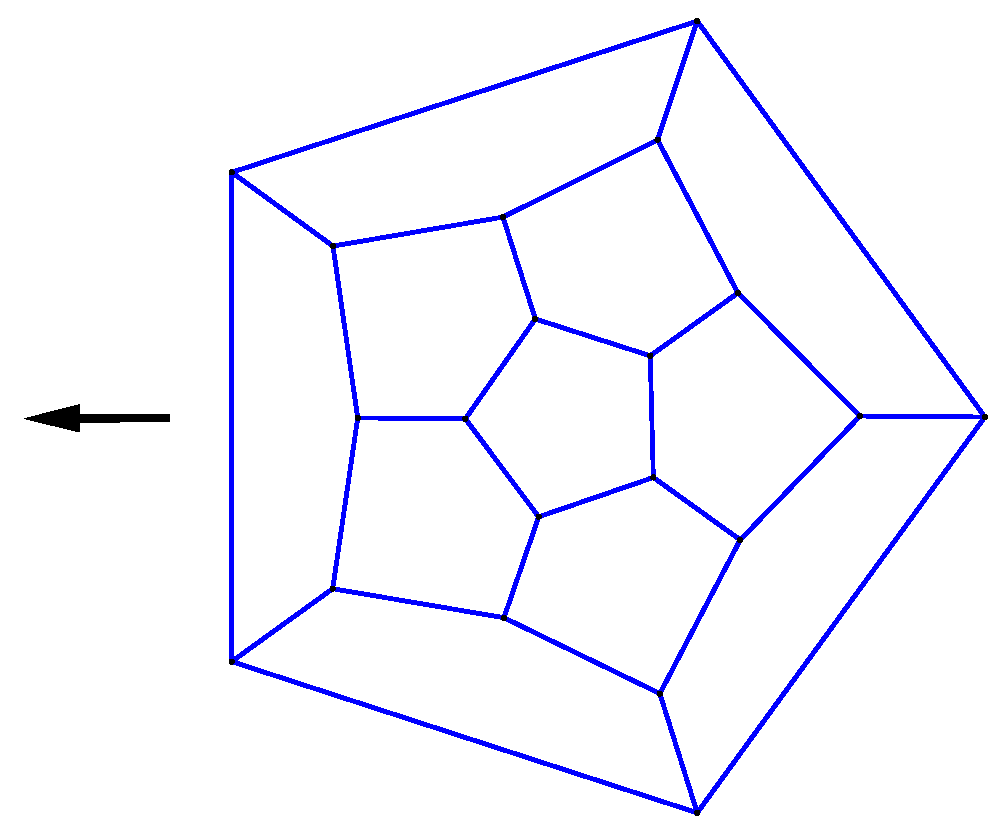
\includegraphics{CanadaPicture/DodecahedronSec.eps}}}\par
\end{minipage}
\begin{minipage}{5.6cm}
\centering
\resizebox{50mm}{!}{\rotatebox{0}{\includegraphics{CanadaPicture/AllOriginalDualMedialDR1.eps}}}\par
\end{minipage}
\end{center}}%
\onlySlide*{2}{\textcolor{red}{$Med(G)=Med(G^*)$}
\begin{center}
\begin{minipage}{5.6cm}
\centering
\resizebox{50mm}{!}{\rotatebox{0}{\includegraphics{CanadaPicture/IcosahedronSec.eps}}}\par
\end{minipage}
\begin{minipage}{5.6cm}
\centering
\resizebox{50mm}{!}{\rotatebox{0}{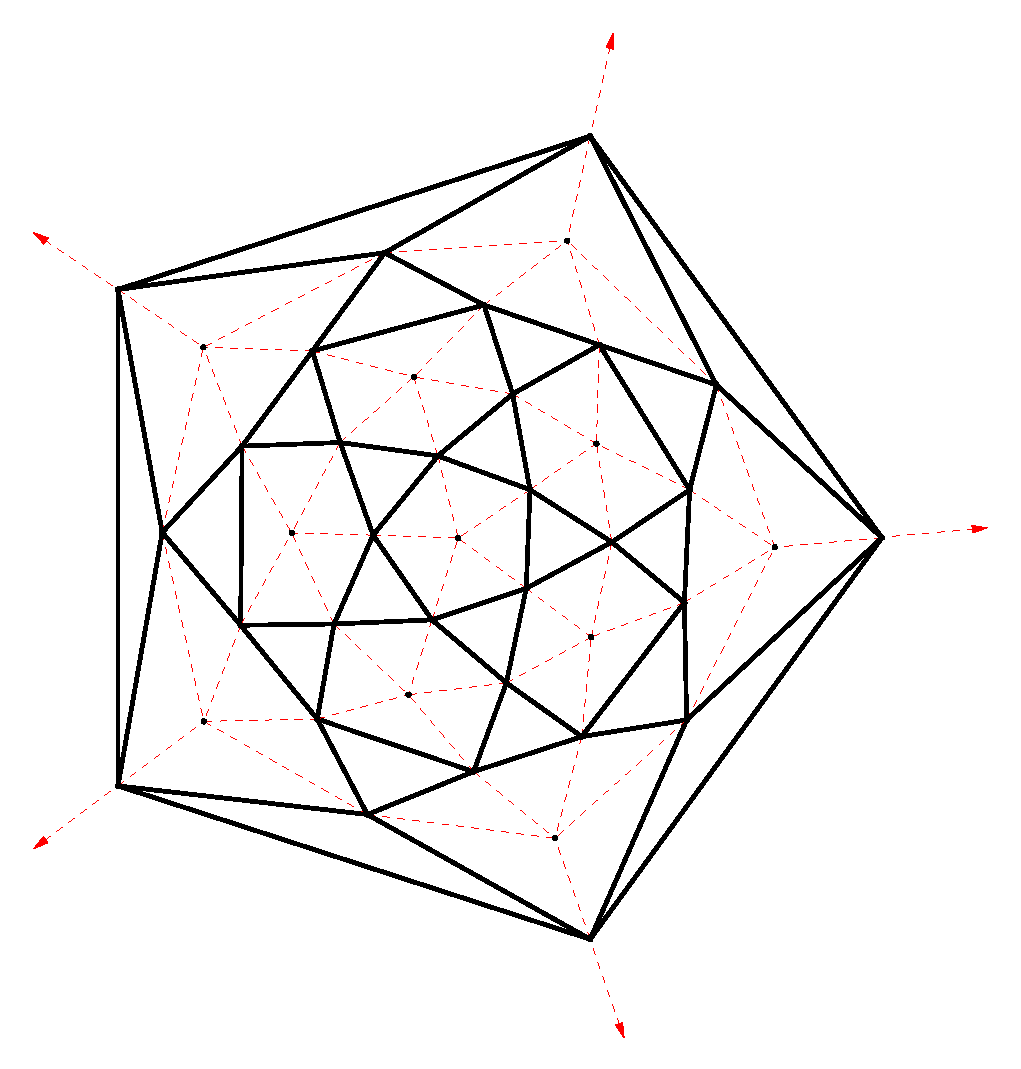
\includegraphics{CanadaPicture/AllOriginalDualMedialDR2.eps}}}\par
\end{minipage}
\end{center}}%

\end{slide}
}



\overlays{3}{
\begin{slide}{Inverse medial graph}
\onlySlide*{1}{
If $G$ is a $4$-valent plane graph, we want to find the graphs $H$ such that $G=Med(H)$.\par
\begin{center}
\begin{minipage}{7.0cm}
\centering
\epsfig{file=CanadaPicture/ChessConstruction1.eps, height=6cm}\par
\end{minipage}
\end{center}}%
\onlySlide*{2}{
Take ${\cal C}_1$(\epsfig{file=CanadaPicture/Square50.eps, height=4mm}), ${\cal C}_2$(\epsfig{file=CanadaPicture/Square00.eps, height=4mm}) a bipartition of the face-set of $G$ or in other word a chess coloring.\par
\begin{center}
\begin{minipage}{7.0cm}
\centering
\epsfig{file=CanadaPicture/ChessConstruction2.eps, height=6cm}\par
\end{minipage}
\end{center}}%
\onlySlide*{3}{
We form two plane graphs $H_{black}$ and $H_{white}$ with the black and white faces.\par
\begin{center}
\begin{minipage}{5.6cm}
\centering
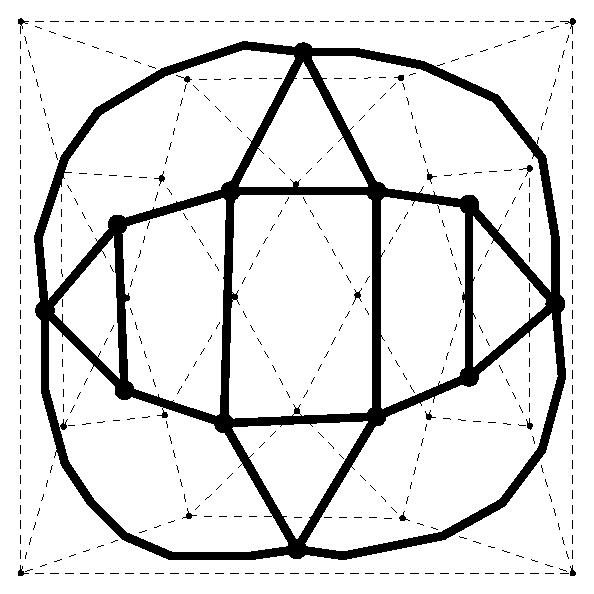
\epsfig{file=CanadaPicture/ChessConstruction3.eps, height=4.5cm}\par
From the \textcolor{red}{black} faces
\end{minipage}
\begin{minipage}{5.6cm}
\centering
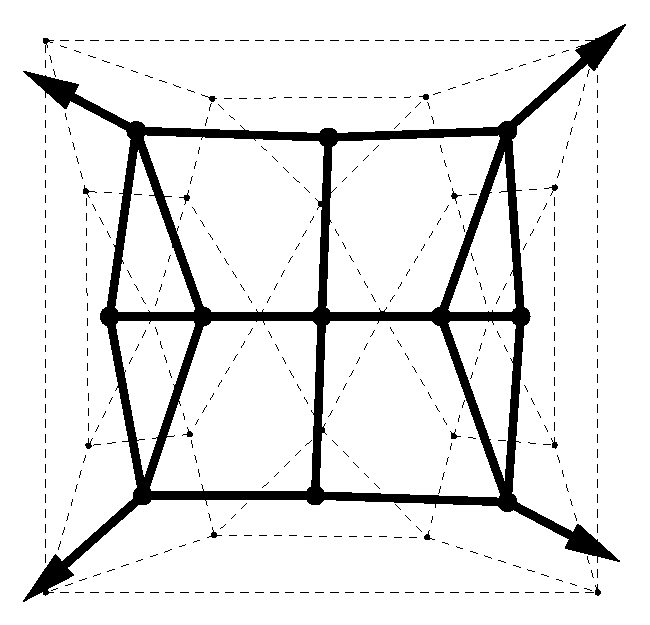
\epsfig{file=CanadaPicture/ChessConstruction4.eps, height=4.5cm}\par
From the \textcolor{red}{white} faces
\end{minipage}
\end{center}
Note that $H_{black}$ can be isomorph to $H_{white}$; $Med(Tetrahedron)=Octahedron$.
}%




\end{slide}
}




%\begin{center}
%\epsfig{file=SequenceGraph.eps,width=10cm}
%\end{center}





\begin{slide}{}
\begin{center}
{\Huge 
\begin{tabular*}{7cm}{c}
\\[-0.3cm]
\textcolor{blue}{II. }\textcolor{red}{Zigzags}\\
\textcolor{red}{and}\\
\textcolor{red}{central circuits}
\end{tabular*}
}
\end{center}
\end{slide}



%%%%%%%%%%%%%%   Central circuits
\overlays{6}{
\begin{slide}{Central circuits}
\onlySlide*{1}{\begin{center}\epsfig{file=GOLDBERGpicture/CentralCircuitSample1.eps,width=10.1cm}\end{center}}%
\onlySlide*{2}{\begin{center}\epsfig{file=GOLDBERGpicture/CentralCircuitSample2.eps,width=10.1cm}\end{center}}%
\onlySlide*{3}{\begin{center}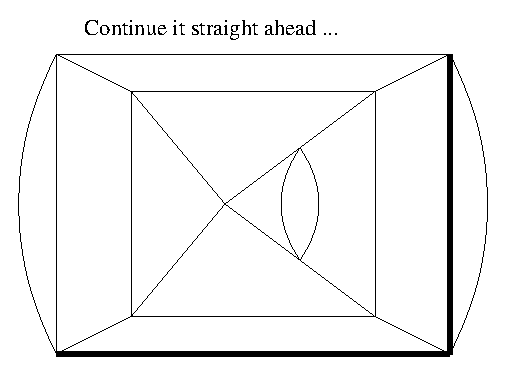
\epsfig{file=GOLDBERGpicture/CentralCircuitSample3.eps,width=10.1cm}\end{center}}%
\onlySlide*{4}{\begin{center}\epsfig{file=GOLDBERGpicture/CentralCircuitSample4.eps,width=10.1cm}\end{center}}%
\onlySlide*{5}{\begin{center}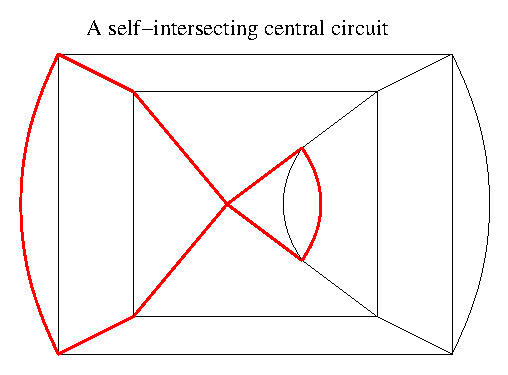
\epsfig{file=GOLDBERGpicture/CentralCircuitSample5.eps,width=10.1cm}\end{center}}%
\onlySlide*{6}{\begin{center}\epsfig{file=GOLDBERGpicture/CentralCircuitSample6.eps,width=9.8cm}\end{center}}%

\end{slide}
}


%%%%%%%%%%%%%%   Zig Zags
\overlays{6}{
\begin{slide}{Zigzags}
\onlySlide*{1}{\begin{center}\epsfig{file=ZIGZAGpicture/ZigZagSample1.eps,width=11cm}\end{center}}%
\onlySlide*{2}{\begin{center}\epsfig{file=ZIGZAGpicture/ZigZagSample2.eps,width=11cm}\end{center}}%
\onlySlide*{3}{\begin{center}\epsfig{file=ZIGZAGpicture/ZigZagSample3.eps,width=11cm}\end{center}}%
\onlySlide*{4}{\begin{center}\epsfig{file=ZIGZAGpicture/ZigZagSample4.eps,width=11cm}\end{center}}%
\onlySlide*{5}{\begin{center}\epsfig{file=ZIGZAGpicture/ZigZagSample5.eps,width=11cm}\end{center}}%
\onlySlide*{6}{\begin{center}\epsfig{file=ZIGZAGpicture/ZigZagSample6.eps,width=9.8cm}\end{center}}%
\end{slide}
}


\overlays{2}{
\begin{slide}{Intersection types for zigzags}
\fromSlide{1}{
\vspace{-2mm}
Let $Z$ and $Z'$ be (possibly, $Z=Z'$) zigzags of a plane
graph $G$ and let an orientation be selected on them. An edge of
intersection $Z\cap Z'$ is called of \textcolor{red}{type I} or \textcolor{red}{type II}, if $Z$ and $Z'$ traverse $e$ in opposite or same direction, respectively
%
%\vspace{2mm}

\begin{center}
\epsfxsize=90mm
\epsfbox{ZIGZAGpicture/TypeI_TypeII-pres.eps}
\end{center}
%
%\vspace{2mm}
}%
\fromSlide{2}{
The types of self-intersection depends on orientation chosen on zigzags except if $Z=Z'$:

\begin{center}
\epsfxsize=80mm
\epsfbox{ZIGZAGpicture/TypeI_TypeIIsec.eps}
\end{center}

}%

\end{slide}
}





\overlays{5}{
\begin{slide}{Intersection types for central circuits}
\onlySlide*{1}{
Let $G$ be a $4$-valent plane graph\par
\begin{center}
\begin{minipage}{7.0cm}
\centering
\epsfig{file=CanadaPicture/ChessConstruction1.eps, height=6cm}\par
\end{minipage}
\end{center}
}%
\onlySlide*{2}{Take ${\cal C}_1$(\epsfig{file=CanadaPicture/Square50.eps, height=4mm}), ${\cal C}_2$(\epsfig{file=CanadaPicture/Square00.eps, height=4mm}) a bipartition of the face-set of $G$\par
\begin{center}
\begin{minipage}{7.0cm}
\centering
\epsfig{file=CanadaPicture/ChessConstruction2.eps, height=6cm}\par
\end{minipage}
\end{center}}%
\onlySlide*{3}{Let $C$ and $C'$ be two central circuits of $G$ and let an orientation be selected on them.
\begin{center}
\begin{minipage}{7.0cm}
\centering
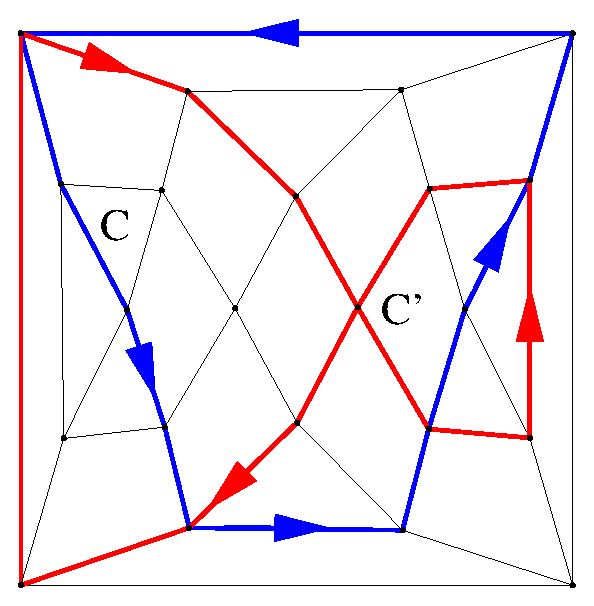
\epsfig{file=CanadaPicture/TwoCentralCircuits.eps, height=6cm}\par
\end{minipage}
\end{center}}%
\onlySlide*{4}{\begin{center}
{ Local View on a vertex $v$ and type}\par
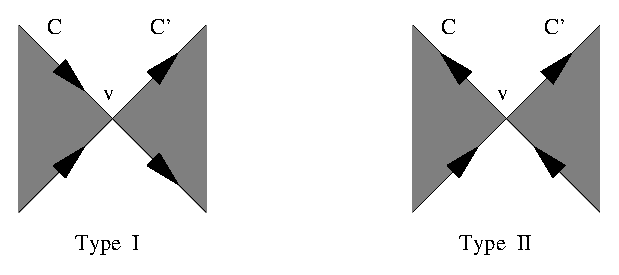
\epsfig{file=CanadaPicture/TypeI_TypeIIccSec.eps, width=10cm}\par
\end{center}

%\begin{center}
%\input{TypeI_TypeIIcc.pstex_t}
%\end{center}
}%
\onlySlide*{5}{$C$ and $C'$ have $2$ intersections I and $2$ intersection II\par
\begin{center}
\begin{minipage}{7.0cm}
\centering
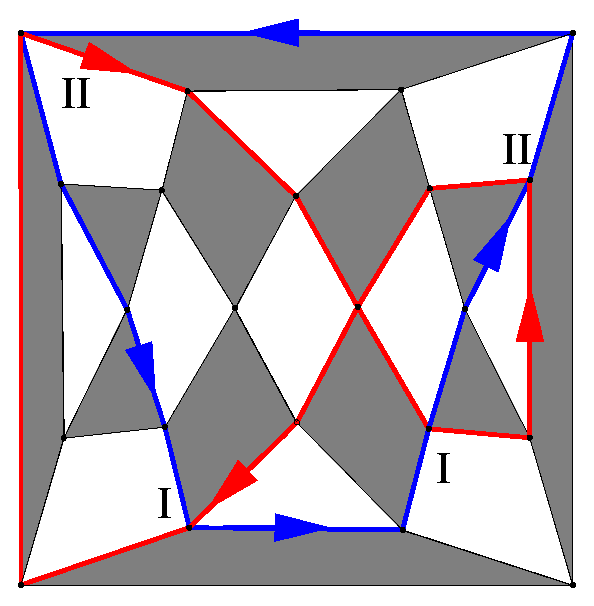
\epsfig{file=CanadaPicture/TwoCentralCircuitsType.eps, height=6cm}\par
\end{minipage}
\end{center}}%
%\onlySlide*{6}{If one interchanges ${\cal C}_1$ and ${\cal C}_2$,
%while keeping the same orientation, then the types of intersection
%of vertices are interchanged.
%
%If $C=C'$, then the type of intersection
%is independent of the chosen orientation; hence,
%the intersection of $C$ with itself, which we will call its
%{\em signature}, relatively to ${\cal C}_1$, ${\cal C}_2$
%is well-defined.
%}%
\end{slide}
}










\overlays{2}{
\begin{slide}{Medial, zigzags and central circuits}
\onlySlide*{1}{\textcolor{red}{Zigzags} of a plane graph \textcolor{blue}{$G$} are in one-to-one correspondence with \textcolor{red}{zigzags} of \textcolor{blue}{$G^*$}.
\begin{center}
\begin{minipage}{5.6cm}
\centering
\resizebox{50mm}{!}{\rotatebox{0}{\includegraphics{CanadaPicture/GrEX1sec.eps}}}\par
\end{minipage}
\begin{minipage}{5.6cm}
\centering
\resizebox{50mm}{!}{\rotatebox{0}{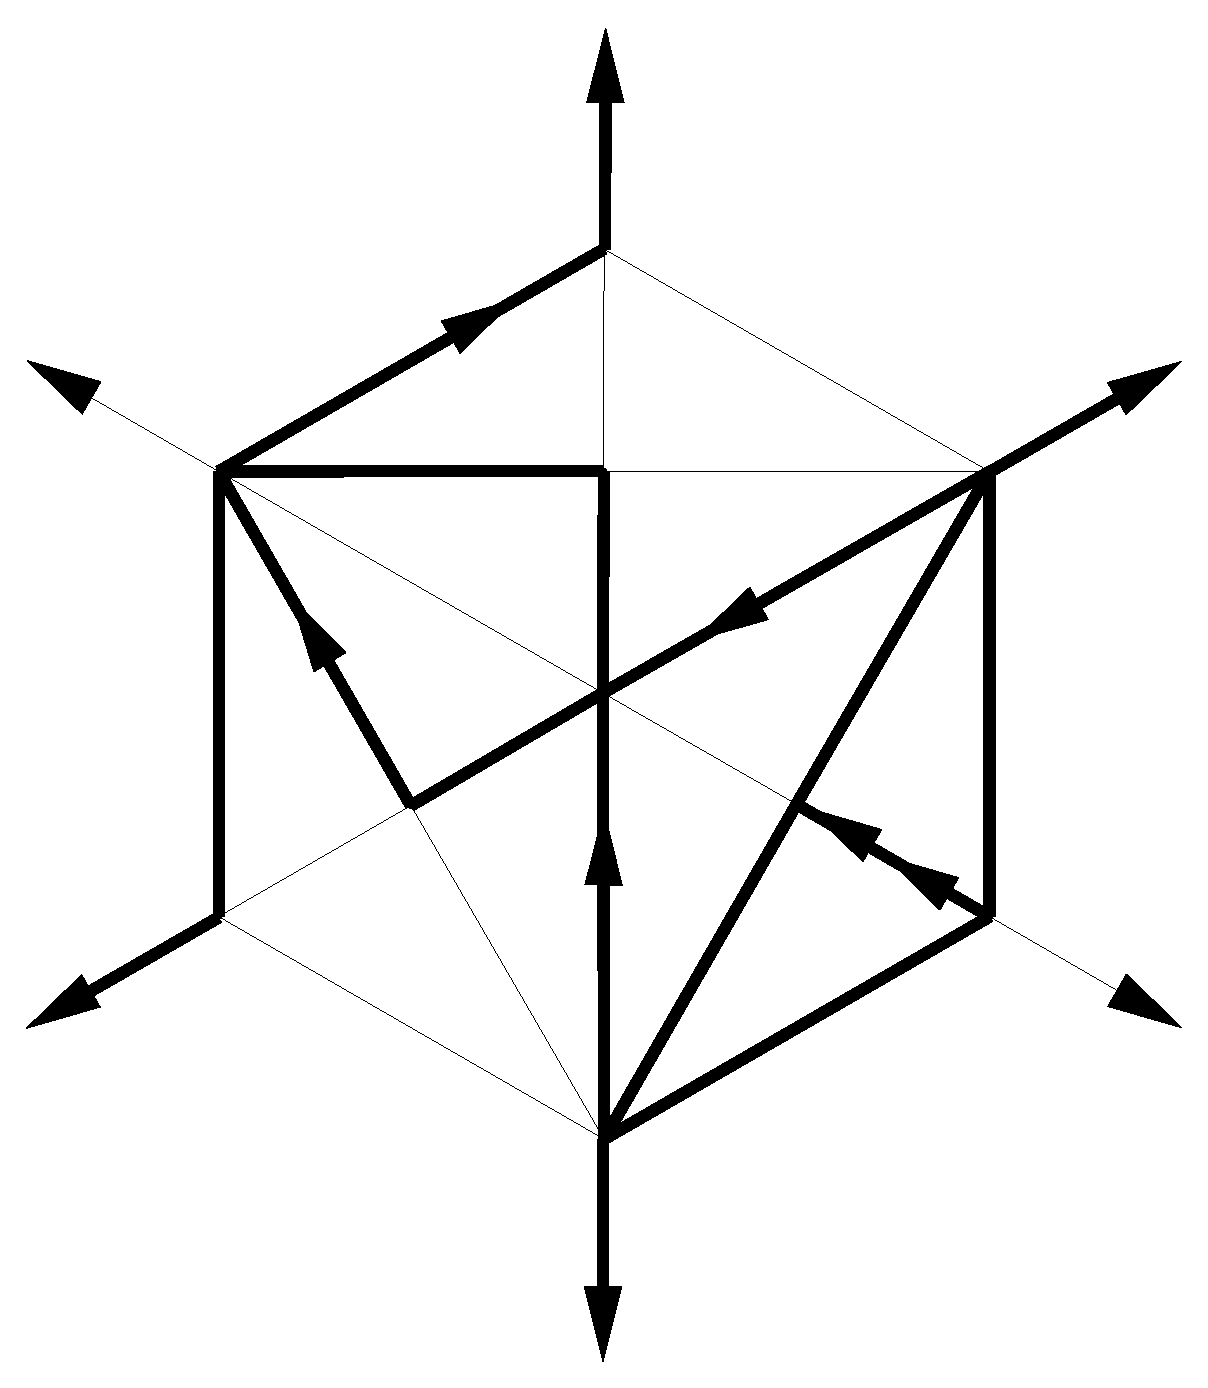
\includegraphics{CanadaPicture/GrEX2sec.eps}}}\par
\end{minipage}
Types are interchanged.
\end{center}}%
\onlySlide*{2}{\textcolor{red}{Zigzags} of a plane graph \textcolor{blue}{$G$} are in one to one correspondence with \textcolor{red}{central circuits} of \textcolor{blue}{$Med(G)$}.
\begin{center}
\begin{minipage}{5.6cm}
\centering
\resizebox{50mm}{!}{\rotatebox{0}{\includegraphics{CanadaPicture/GrEX1sec.eps}}}\par
\end{minipage}
\begin{minipage}{5.6cm}
\centering
\resizebox{50mm}{!}{\rotatebox{0}{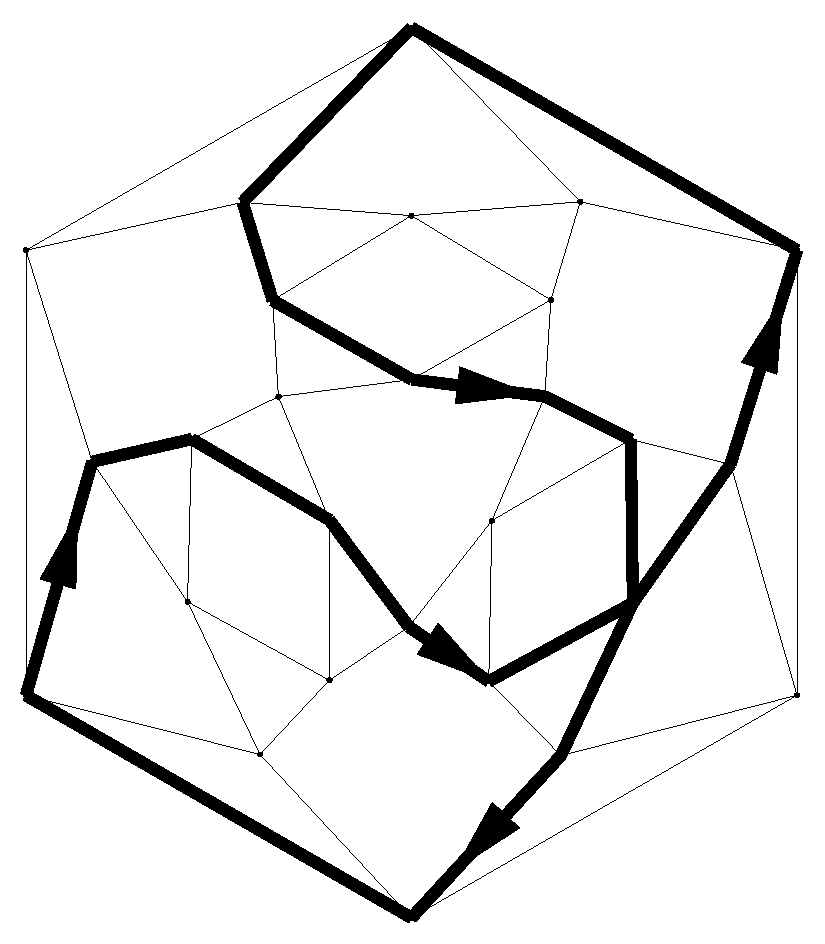
\includegraphics{CanadaPicture/GrEX3sec.eps}}}\par
\end{minipage}
\end{center}}%


\end{slide}
}



%\begin{slide}{Notations}
%\begin{itemize}
%\item \textcolor{red}{ZC-circuit} stands for ``zigzag or central circuit'' in $3$- or $4$-valent plane graphs.
%\vspace{1cm}


%\item The \textcolor{red}{length} of a ZC-circuit is the number of its edges.
%\vspace{1cm}


%\item The \textcolor{red}{ZC-vector} of a $3$- or $4$-valent plane graph $G_0$ is the vector $\dots, c_k^{m_k}, \dots$ where $m_k$ is the number of ZC-circuits of length $c_k$.
%\vspace{1cm}

%\item[\ding{108}] A graph is ZC-transitive if its group of automorphism is transitive on the set of ZC-circuits
%\item Zigzags of a graph $G$ correspond to central circuits of the medial $Med(G)$.
%\end{itemize}
%\end{slide}







%\begin{slide}{Zigzag parameters}
%\begin{enumerate}
%\item[\ding{108}] The \textcolor{red}{signature} of a zigzag $Z$ is
%the pair $(\alpha_1,\alpha_2)$, where $\alpha_1$ and $\alpha_2$ are the
%numbers of its edges of self-intersection of type I and type II, respectively.
%
%\vspace{1mm}
%
%\item[\ding{108}] The \textcolor{red}{intersection vector $Int(Z)$} lists
%pairs of intersection $(\alpha_1, \alpha_2)$ with all other zigzags.
%
%\vspace{1mm}
%
%\item[\ding{108}] \textcolor{red}{z-vector} of $G$ is the
%vector enumerating \textcolor{red}{lengths} (numbers of edges) of all its
%zigzags with their signature as subscript.
%
%\item[\ding{108}] All intersections are even for maps on sphere. This no longer true for maps on surfaces of genus $g\geq 1$.
%
%\end{enumerate}
%
%\begin{center}
%\begin{minipage}{3cm}
%\epsfxsize=25mm
%\epsfbox{Graph12_6sec.eps}
%\end{minipage}
%\begin{minipage}{7cm}
%$2$ zigzags with $Int=(1,3), (3,3)$\\
%$1$ self-intersecting with $Int=(3,3)^{2}$
%\end{minipage}
%\end{center}
%
%\end{slide}



\begin{slide}{Intersection two simple ZC-circuits}
\vspace{-3mm}
\begin{itemize}
%\item Intersection of two ZC-circuits for $3$- or $4$-valent plane graphs is always even.
\item For the class of \textcolor{red}{graph $4_n$} the size of the intersection of two simple zigzags belongs to \textcolor{red}{$\{0,2,4,6\}$}.
\item For classes of \textcolor{red}{octahedrites}, \textcolor{red}{graph $3_n$} or \textcolor{red}{graph $5_n$} the size of the intersection of two simple ZC-circuits can be any \textcolor{red}{even number}.
%\item 
\end{itemize}
\begin{center}
\begin{minipage}{7cm}
\centering
\vspace{-5mm}
\epsfig{figure=ZIGZAGpicture/ConstructionH8thisec-color.eps,height=5cm}
\end{minipage}
\begin{minipage}{4cm}
Two simple zigzags of a graph \textcolor{red}{$5_n$} with \textcolor{red}{$|Z\cap Z'|=8$}.\par
\vspace{1cm}
On surfaces of genus $g\geq 1$, the intersection can be odd.
\end{minipage}

\end{center}


\end{slide}







%\begin{slide}{Duality and types}
%\vspace{2mm}
%
%{\em {\bf Theorem}
%
%Let $G$ be a plane graph; for any orientation of all zigzags of $G$, we have:
%
%(i) The number of edges of type II, which are incident to any fixed \textcolor{red}{vertex}, is even.
%
%(ii) The number of edges of type I, which are incident to any fixed \textcolor{red}{face}, is even.
%}


%\end{slide}





\begin{slide}{Bipartite graphs}

\vspace{-2mm}

{\em {\bf Remark}
A plane graph is \textcolor{red}{bipartite} if and only if its faces have even gonality.
}



{\em {\bf Theorem} (\textcolor{blue}{Shank-Shtogrin})

For any planar bipartite graph $G$ there exist an orientation of zigzags, with respect to which each edge has type I.
}


\begin{center}
\begin{minipage}{5.5cm}
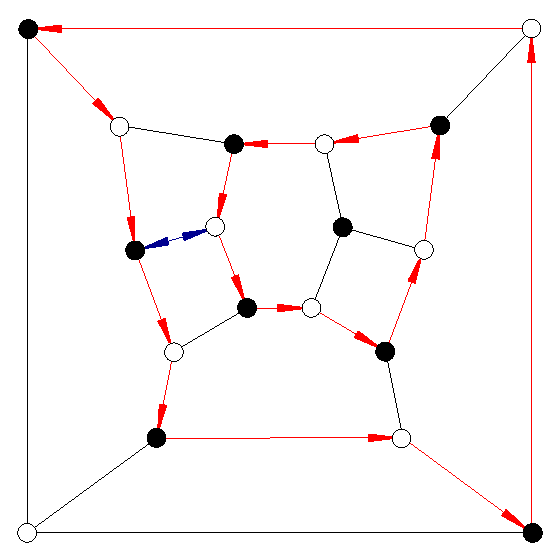
\epsfig{file=ZIGZAGpicture/ExampleBipartitionSec2.eps, width=5cm}
\end{minipage}
\begin{minipage}{3cm}
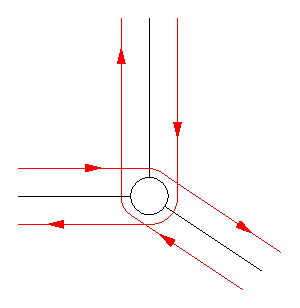
\epsfig{file=ZIGZAGpicture/LocalDraw.eps, width=3cm}
\end{minipage}
\end{center}

\end{slide}







%\begin{slide}{Zigzag properties of a graph}
%{\scriptsize
%\begin{enumerate}
%\item[\ding{108}] \textcolor{red}{$z$-uniform}: all zigzags have the same length and signature, 
%\item[\ding{108}] \textcolor{red}{$z$-transitive}: symmetry group is transitive on zigzags,
%\item[\ding{108}] \textcolor{red}{$z$-knotted}: there is only one zigzag,
%\item[\ding{108}] \textcolor{red}{$z$-balanced}: all zigzags of the same length and signature, have identical intersection vectors.
%\end{enumerate}
%}
%All known $z$-uniform $3$-valent graphs are $z$-balanced.
%
%\begin{center}
%\begin{minipage}[b]{3.7cm}
%\centering
%\epsfig{figure=FirstUnbalancedTrig.eps,height=2cm}\par
%{\tiny $18$-vertices $(C_2)$, $z=8^3; 30_{2,5}$}
%\end{minipage}
%\begin{minipage}[b]{3.7cm}
%\centering
%\epsfig{figure=FirstUnbalanced4n.eps,height=2cm}\par
%{\tiny $4_{72}$($C_1$), $z=30_{1,0}, 54^2_{4,0}, 78_{13, 0}$}
%\end{minipage}
%\begin{minipage}[b]{3.7cm}
%\centering
%\epsfig{figure=FirstUnbalanced5n.eps,height=2cm}\par
%{\tiny $5_{52}$($D_{2d}$),\par
% $z=16^4; 92_{12, 12}$}
%\end{minipage}
%\end{center}
%\vspace{-2mm}
%\begin{center}
%{\tiny Smallest (among all $3$-valent, all $4_n$, all $5_n$) $z$-unbalanced $3$-valent graphs}
%\end{center}
%\end{slide}







%\begin{slide}{Zigzags of reg. and semireg. polyhedra}
%
%\begin{center}
%{\scriptsize
%\begin{tabular}{||c|c|c|c||}
%\hline
%\hline
%\#\,edges&polyhedron& $z$-vector&int. vector \\ \hline
%\hline
%6  &\textcolor{red}{Tetrahedron}&$4^3$&$(1,1)^2$\\ 
%12 &\textcolor{red}{Cube, Octahedron}&$6^4$&$(0,2)^3$\\ 
%%12 &\textcolor{red}{Octahedron}&$6^4$&$2^3$\\ 
%30 &\textcolor{red}{Dodecahedron, Icosahedron}&$10^6$&$(0,2)^5$\\\hline
%%30 &\textcolor{red}{Icosahedron}&$10^6$&$2^5$\\ \hline
%24 &\textcolor{red}{Cuboctahedron}&$8^6$&$(0,2)^4,(0,0)$ \\%=Med(cube)=Med(octahedron)
%60 &\textcolor{red}{Icosidodecahedron}&$10^{12}$&$(0,2)^5,(0,0)^6$ \\%=Med(ico.)=Med(dode.)
%48 &\textcolor{red}{Rhombicuboctahedron}&$12^8$&$(0,2)^6,(0,0)$\\ %=Med(cuboctahedron)
%120&\textcolor{red}{Rhombicosidodecahedron}&$20^{12}$&$(0,2)^{10},(0,0)$\\ %=Med(icosidodecahedron)
%72 &\textcolor{red}{Truncated Cuboctahedron}&$18^8$&$(0,6),(0,2)^6$\\ 
%180&\textcolor{red}{Truncated Icosidodecahedron}&$30^{12}$&$(0,10),(0,2)^{10}$\\ 
%18 &\textcolor{red}{Truncated Tetrahedron}&$12^3$&$(3,3)^2$\\ 
%36 &\textcolor{red}{Truncated Octahedron}&$12^6$&$(0,4),(0,2)^4$\\ 
%\hline
%\hline
%\end{tabular}
%}
%\end{center}
%\end{slide}






%\begin{slide}{}
%
%\begin{center}
%{\scriptsize
%\begin{tabular}{||c|c|c|c||}
%\hline
%\hline
%36 &\textcolor{red}{Truncated Cube}&$18^4$&$(2,4)^3$\\
%90 &\textcolor{red}{Truncated Icosahedron}&$18^{10}$&$(0,2)^9$\\ 
%90 &\textcolor{red}{Truncated Dodecahedron}&$30^6$&$(2,4)^5$\\ 
%60 &\textcolor{red}{Snub Cube}&$30_{3,0}^4$&$(4,4)^3$\\ 
%150&\textcolor{red}{Snub Dodecahedron}&$50_{5,0}^6$&$(4,4)^5$\\ \hline
%3m &$Prism_m$, $m\equiv 0 \pmod{4}$&$(\frac{3m}{2})^4$&$(0,\frac{m}{2})^3$\\
%3m &$Prism_m$, $m\equiv 2 \pmod{4}$&$({3m}_{\frac{m}{2},0})^2$&$(0,2m)$\\ 
%3m &$Prism_m$, $m\equiv 1,3 \pmod{4}$&${6m}_{m,2m}$&\\ 
%4m &$APrism_m, m \equiv 0 \pmod{3}$&$(2m)^4$&$(0,\frac{2m}{3})^3$\\ 
%4m &$APrism_m, m \equiv 1,2 \pmod{3}$&$2m;6m_{0,2m}$&\\ \hline\hline
%84 &\textcolor{red}{Klein map}(oriented, genus $3$ surface)&$8^{21}$&$(0,1)^8, {0}^{12}$\\
%48 &\textcolor{red}{Dyck map}(oriented, genus $3$ surface)&$6^{16}$&$(0,1)^6, {0}^9$\\
%\hline
%\hline
%\end{tabular}
%}
%\end{center}
%\end{slide}







%\begin{slide}{First generalizations of zigzags}
%\vspace{3mm}
%
%Above Table contains plane graphs, which are not $3$-valent, and non-planar graphs.
%
%\vspace{6mm}
%
%In fact, the notion of zigzag can be easily generalized on any \textcolor{blue}{plane graph} and on a graph, embedded in any \textcolor{blue}{oriented surface}.
%
%\vspace{6mm}
%
%Moreover, this notion, being local, can be generalized even for \textcolor{blue}{non-oriented surfaces}.
%
%\end{slide}



%\begin{slide}{Perfect matching on $5_n$ graphs}
%\vspace{-4mm}
%\begin{center}
%\begin{minipage}{57mm}
%{\scriptsize
%Let $G$ be a graph $5_n$ with \textcolor{red}{one zigzag} with self-intersection numbers $(\alpha_1, \alpha_2)$.
%\begin{enumerate}
%\item[(i)] $\alpha_1\geq \frac{n}{2}$. If $\alpha_1=\frac{n}{2}$ then the edges of self-intersection of type I form a \textcolor{red}{perfect matching} $PM$
%\item[(ii)] every face incident to \textcolor{red}{$0$ or $2$} edges of $PM$
%\item[(iii)] two faces, $F_1$ and $F_2$ are free of $PM$, $PM$ is organized around them in \textcolor{red}{concentric circles}.
%\end{enumerate}
%}
%\end{minipage}
%\begin{minipage}{5.5cm}
%\epsfxsize=55mm
%\epsfbox{ZZkekule34sec.eps}
%\end{minipage}
%\end{center}
%
%{\scriptsize
%
%M. Deza, M. Dutour and P.W. Fowler, {\em Zigzags, Railroads and Knots in Fullerenes}, Journal of Chemical Information and Computer Sciences, in press.
%}
%
%\end{slide}






%\begin{slide}{}
%\begin{center}
%{\Huge 
%\begin{tabular*}{10cm}{c}
%\\[-1.2cm]
%\textcolor{blue}{III. }\textcolor{red}{Four Tables}\\
%\textcolor{red}{on zigzags notions}\\
%\textcolor{red}{for fullerenes $5_n$}\\
%{\large \textcolor{red}{(from Deza, Dutour and Fowler)}}
%\end{tabular*}
%}
%\end{center}
%
%\end{slide}





%\begin{slide}{$z$-uniform $5_n$ with $n\leq 60$}
%\vspace{-7mm}
%\begin{center}
%{\tiny
%\begin{tabular}{|c||c|c|c|c|}
%\hline
%$\,\,n$&isomer    &orbit lengths& $z$-vector    &  int. vector\\
%\hline
%$20$& $I_h$:1     &$6$         &$10_{0,0}^6$   &  $2\sp{5}$\\
%$28$& $T_d$:2     &$4$,$3$     &$12_{0,0}^7$   &  $2\sp{6}$\\
%$40$& $T_d$:40    &$4$         &$30_{0,3}^4$   &  $8\sp{3}$\\
%$44$& $T$:73      &$3$         &$44_{0,4}^3$   &  $18\sp{2}$\\
%$44$& $D_2$:83    &$2$         &$66_{5,10}^2$  &  $36$\\
%$48$& $C_2$:84    &$2$         &$72_{7,9}^2$   &  $40$\\
%$48$& $D_3$:188   &$3$,$3$,$3$ &$16_{0,0}^9$   &  $2\sp{8}$\\
%$52$& $C_3$:237   &$3$         &$52_{2,4}^3$   &  $20\sp{2}$\\
%$52$& $T$:437     &$3$         &$52_{0,8}^3$   &  $18\sp{2}$\\
%$56$& $C_2$:293   &$2$         &$84_{7,13}^2$  &  $44$\\
%$56$& $C_2$:349   &$2$         &$84_{5,13}^2$  &  $48$\\
%$56$& $C_3$:393   &$3$         &$56_{3,5}^3$   &  $20\sp{2}$\\
%$60$& $C_2$:1193  &$2$         &$90_{7,13}^2$  &  $50$\\
%$60$& $D_2$:1197  &$2$         &$90_{13,8}^2$  &  $48$\\
%\textcolor{red}{$60$}& $D_3$:1803  &$6$,$3$,$1$ &\textcolor{red}{$18_{0,0}^{10}$}&  \textcolor{red}{$2\sp{9}$}\\
%\textcolor{blue}{$60$}& $I_h$:1812  &$10$        &\textcolor{blue}{$18_{0,0}^{10}$}&  \textcolor{blue}{$2\sp{9}$}\\
%\hline
%\end{tabular}
%}
%\end{center}

%\begin{center}
%All $z$-uniform $5_n$ with $n\leq 60$ (DDF)
%\end{center}
%
%\begin{enumerate}
%\item M. Deza, M. Dutour and P.W. Fowler, {\em Zigzags, Railroads and Knots in Fullerenes}, (2002).
%\end{enumerate}


%\end{slide}





%\begin{slide}{$z$-uniform \textcolor{red}{IPR} $5_n$ with $n\leq 100$}
%
%\begin{center}
%{\tiny
%\begin{tabular}{|c||c|c|c|c|}
%\hline
%$\,\,n$&isomer    &orbit lengths& $z$-vector    &  int. vector\\
%\hline
%$80$&$I_h$:7    &$12$   &$20_{0,0}^{12}$ &$0,2\sp{10}$\\
%\textcolor{red}{$84$}&$T_d$:20   &$6$    &\textcolor{red}{$42_{0,1}^{6}$}  &\textcolor{red}{$8\sp{5}$}\\
%\textcolor{blue}{$84$}&$D_{2d}$:23&$4$,$2$&\textcolor{blue}{$42_{0,1}^{6}$}  &\textcolor{blue}{$8\sp{5}$}\\
%$86$&$D_3$:19   &$3$    &$86_{1,10}^{3}$ &$32\sp{2}$\\
%$88$&$T$:34     &$12$   &$22_{0,0}^{12}$ &$2\sp{11}$\\
%$92$&$T$:86     &$6$    &$46_{0,3}^6$    &$8\sp{5}$\\
%$94$&$C_3$:110  &$3$    &$94_{2,13}^3$   &$32\sp{2}$\\
%$100$&$C_2$:387 &$2$    &$150_{13,22}^2$ &$80$\\
%$100$&$D_2$:438 &$2$    &$150_{15,20}^2$ &$80$\\
%\textcolor{red}{$100$}&\textcolor{red}{$D_2$}:432 &\textcolor{red}{$2$}    &\textcolor{red}{$150_{17,16}^2$} &\textcolor{red}{$84$}\\
%\textcolor{blue}{$100$}&\textcolor{blue}{$D_2$}:445 &\textcolor{blue}{$2$}    &\textcolor{blue}{$150_{17,16}^2$} &\textcolor{blue}{$84$}\\
%\hline
%\end{tabular}
%}
%\end{center}
%\textcolor{red}{IPR} means the absence of adjacent pentagonal faces;
%
%IPR enhanced stability of putative fullerene molecule.


%\begin{center}
%All $z$-uniform $5_n$ with $n\leq 60$ (DDF)
%\end{center}
%
%\begin{enumerate}
%\item M. Deza, M. Dutour and P.W. Fowler, {\em Zigzags, Railroads and Knots in Fullerenes}, (2002).
%\end{enumerate}
%\end{slide}







%\begin{slide}{IPR $z$-knotted $5_n$ with $n\leq 100$}
%\begin{center}
%\begin{minipage}{5.5cm}
%{\tiny
%\begin{tabular}{|c||c|c|}
%\hline
%$\,\,n$  &signature &isomers\\
%\hline
%86       &$43,86^{\textcolor{red}{*}}$&$C_2$:$2$\\
%90       &$47,88$&$C_1$:$7$\\
%         &$53,82$&$C_2$:$19$\\
%         &$71,64$&$C_2$:$6$\\
%94       &$47,94^{\textcolor{red}{*}}$&$C_1$:$60$; $C_2$:$26$, $126$\\
%         &$65,76$&$C_2$:$121$\\
%         &$69,72$&$C_2$:$7$\\
%96       &$49,95$&$C_1$:$65$\\
%         &$53,91$&$C_1$:$7$, $37$, $63$\\
%\hline
%\end{tabular}
%}
%\end{minipage}
%\begin{minipage}{5.5cm}
%{\tiny
%\begin{tabular}{|c||c|c|}
%\hline
%98       &$49,98^{\textcolor{red}{*}}$&$C_2$:$191$, $194$, $196$\\
%         &$63,84$&$C_1$:$49$\\
%         &$75,72$&$C_1$:$29$\\
%         &$77,70$&$C_1$:$5$; $C_2$:$221$\\
%100      &$51,99$&$C_1$:$371$, $377$; $C_3$:$221$\\
%         &$53,97$&$C_1$:$29$, $113$, $236$\\
%         &$55,95$&$C_1$:$165$\\
%         &$57,93$&$C_1$:$21$\\
%         &$61,89$&$C_1$:$225$\\
%         &$65,85$&$C_1$:$31$, $234$\\
%\hline
%\end{tabular}
%}
%\end{minipage}
%\end{center}
%The symbol \textcolor{red}{${}^*$} above means that fullerene forms a \textcolor{red}{K\'ekule structure}, i.e. edges of self-intersection of type I cover exactly once the vertex-set of the fullerene graph (in other words, they form a \textcolor{red}{perfect matching} of the graph).
%
%
%\end{slide}



%\begin{slide}{Statistics of $z$-knotted $5_n$ with $n\leq 74$}
%\begin{center}
%\begin{minipage}{4.5cm}
%{\tiny
%\begin{tabular}{|c||c|c|}
%\hline
%$\,\,n$  &\# of $5_n$&\# of $z$-knotted\\
%\hline
%$34$&    $6$&$1$\\
%$36$&   $15$&$0$\\
%$38$&   $17$&$4$\\
%$40$&   $40$&$1$\\
%$42$&   $45$&$6$\\
%$44$&   $89$&$9$\\
%$46$&  $116$&$15$\\
%$48$&  $199$&$23$\\
%$50$&  $271$&$30$\\
%$52$&  $437$&$42$\\
%\hline
%\end{tabular}
%}
%\end{minipage}
%\begin{minipage}{3.5cm}
%{\tiny
%\begin{tabular}{|c||c|c|}
%\hline
%$54$&  $580$&$93$\\
%$56$&  $924$&$87$\\
%$58$& $1205$&$186$\\
%$60$& $1812$&$206$\\
%$62$& $2385$&$341$\\
%$64$& $3465$&$437$\\
%$66$& $4478$&$567$\\
%$68$& $6332$&$894$\\
%$70$& $8149$&$1048$\\
%$72$&$11190$&$1613$\\
%$74$&$14246$&$1970$\\
%\hline
%\end{tabular}
%}
%\end{minipage}
%\end{center}
%It will be interesting to estimate the relative order of magnitude of $z$-knotted fullerenes among all $5_n$ and of $z$-knotted $3$-valent graphs among all of them.
%
%\end{slide}








\begin{slide}{}
\begin{center}
{\Huge 
\begin{tabular*}{6.2cm}{c}
\\[-0.6cm]
\textcolor{blue}{III. }\textcolor{red}{Railroad}\\
\textcolor{red}{structure}\\
\textcolor{red}{and tightness}
\end{tabular*}
}
\end{center}
\end{slide}


%\begin{slide}{}
%\begin{center}
%{\Huge
%\begin{tabular*}{6cm}{c}
%\\[-0.5cm]
%\textcolor{blue}{V. }\textcolor{red}{Tightness}\\
%\textcolor{red}{and}\\
%\textcolor{red}{Extremal problems}
%\end{tabular*}
%}
%\end{center}
%\end{slide}






%\begin{slide}{Railroads with triple points in small $4_n$}
%
%\vspace{-2mm}
%\begin{center}
%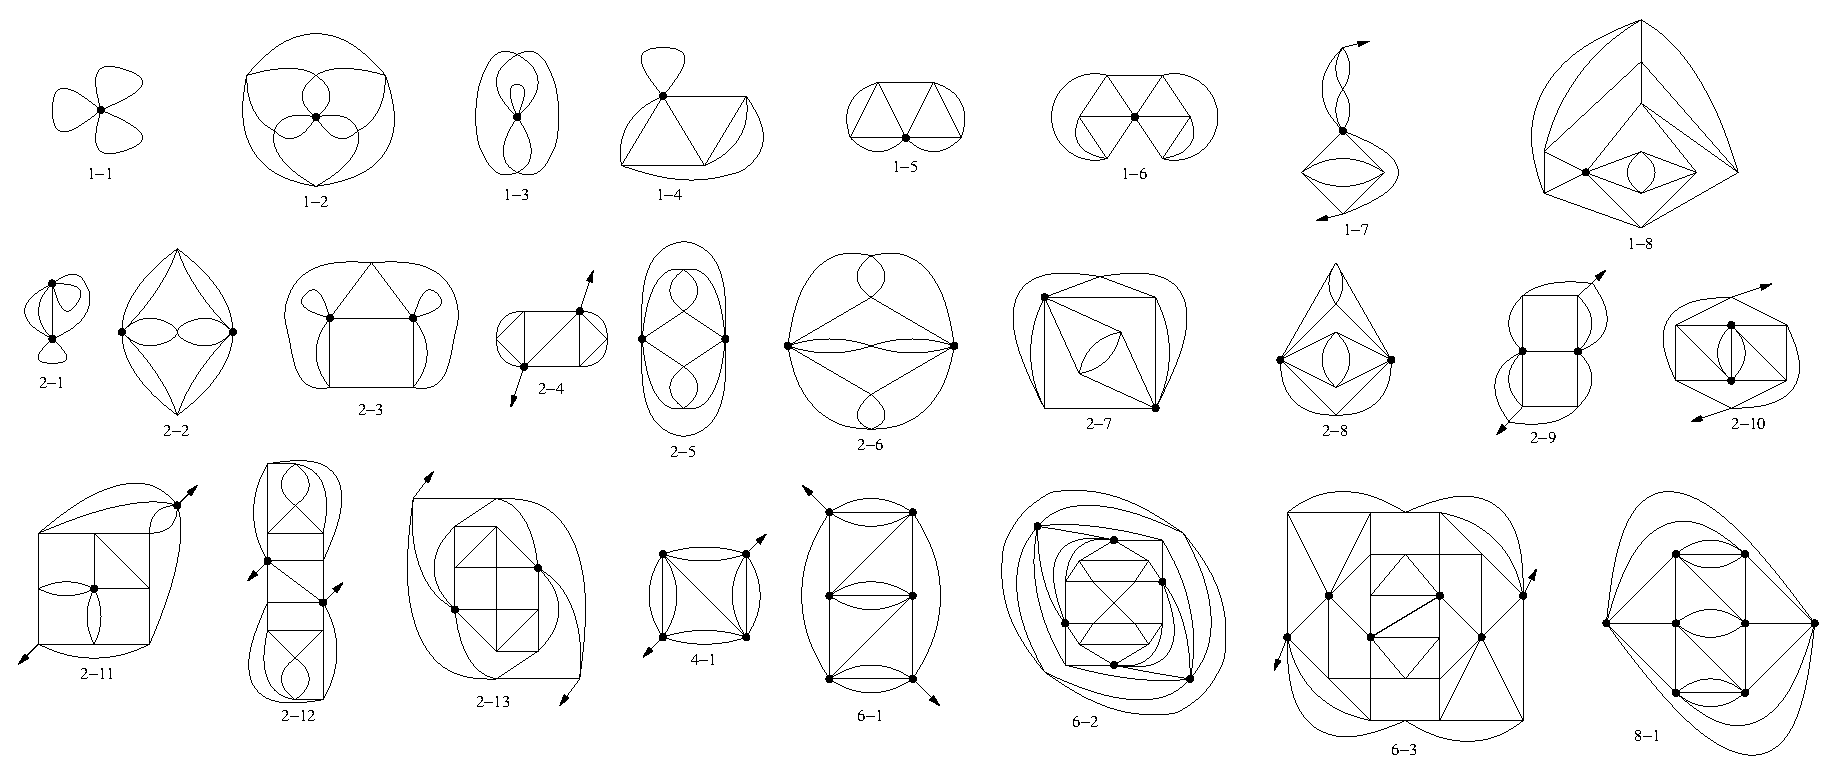
\epsfig{file=CurveByTripleRailroad.eps, height=7cm}
%\end{center}
%
%\end{slide}














%\begin{slide}{First IPR $5_n$ with self-intersect. railroad}
%\begin{center}
%\centering
%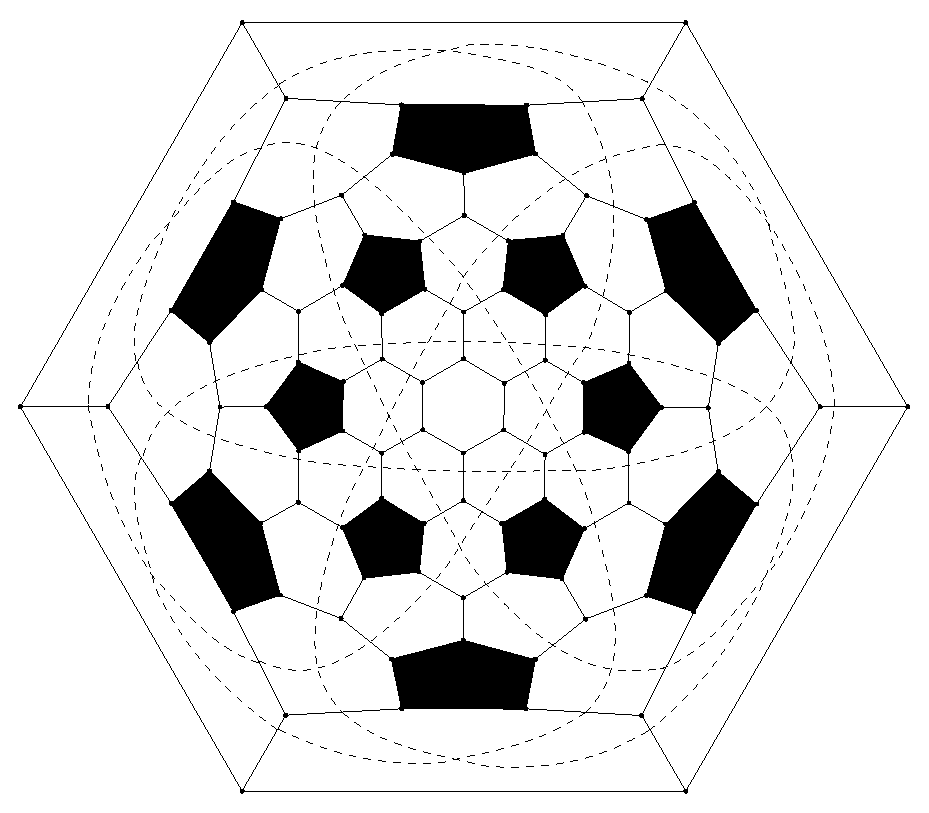
\epsfig{file=DoorDraw.eps, height=75mm}\par
%\end{center}
%\end{slide}
%










%\begin{slide}{Hexagon-triangle adjacencies for $3_n$}
%\vspace{-2mm}
%\begin{enumerate}
%\item[\ding{108}] no hexagon is adjacent to $\leq 2$ triangles; two cases:
%\begin{center}
%\begin{minipage}{3.5cm}
%\epsfig{file=Tetrahedron.ps, height=1.5cm}
%\end{minipage}
%\begin{minipage}{3.5cm}
%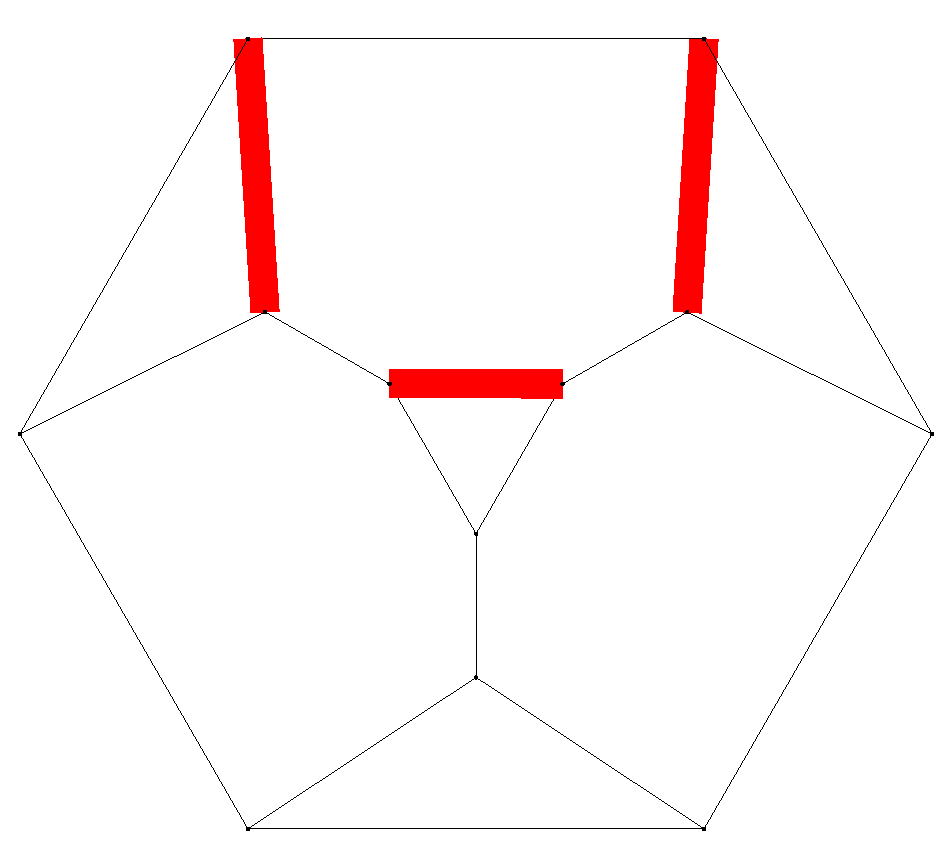
\epsfig{file=TruncatedTetrahedronSec.eps, height=1.5cm}
%\end{minipage}
%\end{center}
%\item[\ding{108}] any hexagon is adjacent to $0$ or $2$ triangles; two series
%\begin{center}
%\begin{minipage}[b]{2.5cm}%
%\centering
%\epsfig{figure=Graphiii24sec.eps,height=1.7cm}
%\end{minipage}
%\begin{minipage}[b]{2.5cm}%
%\centering
%\epsfig{figure=Graphiii28sec.eps,height=1.7cm}
%;
%\end{minipage}
%\begin{minipage}[b]{2.5cm}%
%\centering
%\epsfig{figure=First3nD2.sec.eps,height=1.7cm}
%\end{minipage}
%\begin{minipage}[b]{2.5cm}%
%\centering
%\epsfig{figure=Bigam32_2sec.eps,height=1.7cm}
%\end{minipage}
%\end{center}
%%some hexagons are adjacent to $1$ triangle
%\item[\ding{108}] others give a $5_n$ by collapsing of triangles
%\begin{center}
%\epsfig{file=FowlerConstruction.eps, height=1.3cm}
%\end{center}
%
%\end{enumerate}
%
%\end{slide}









%\begin{slide}{Railroads and pseudo-roads of $4_{126}(D_{3h})$}
%
%\begin{center}
%\begin{minipage}[b]{5.6cm}%
%\centering
%\epsfig{figure=RailRoadSystemCurveSelf.eps,height=4.5cm}\par
%{\scriptsize One of two self-intersecting railroads and the equatorial simple railroad}
%\end{minipage}
%\begin{minipage}[b]{5.5cm}%
%\centering
%\epsfig{figure=RailRoadSystemPseudo.eps,height=5cm}\par
%{\scriptsize All twelve pseudo-roads}
%\end{minipage}
%\end{center}
%A \textcolor{red}{pseudo-road} between $4$-gons $b$ and $c$ is a sequence of
%hexagons $a_1$, \dots, $a_l$,
%s.t. if $a_0=b$ and $a_{l+1}=c$, then any $a_i$,
%$1\leq i\leq l$, is adjacent to $a_{i-1}$ and $a_{i+1}$ on
%opposite edges.
%\end{slide}


\begin{slide}{Railroads, $4$-valent case}
A \textcolor{red}{railroad} in an octahedrite is a circuit of square faces, such that any of them is adjacent to its neighbors on opposite faces. Any railroad is bordered by two central circuits.

\begin{center}
\begin{minipage}{5.5cm}
\centering
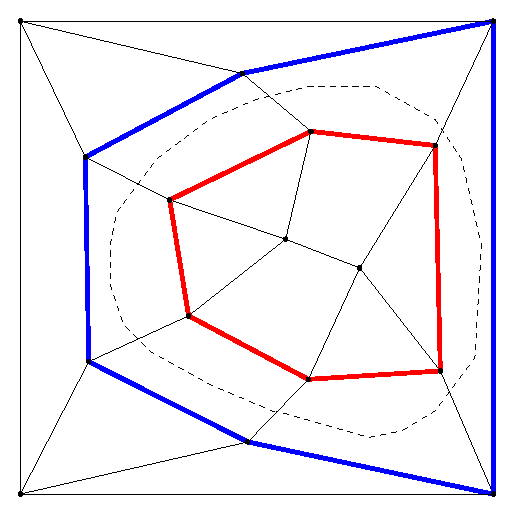
\epsfig{file=CanadaPicture/ExampleRedSec.eps, height=4cm}\par
%$oc_{16}(D_{2})$
\end{minipage}
\begin{minipage}{5.5cm}
\centering
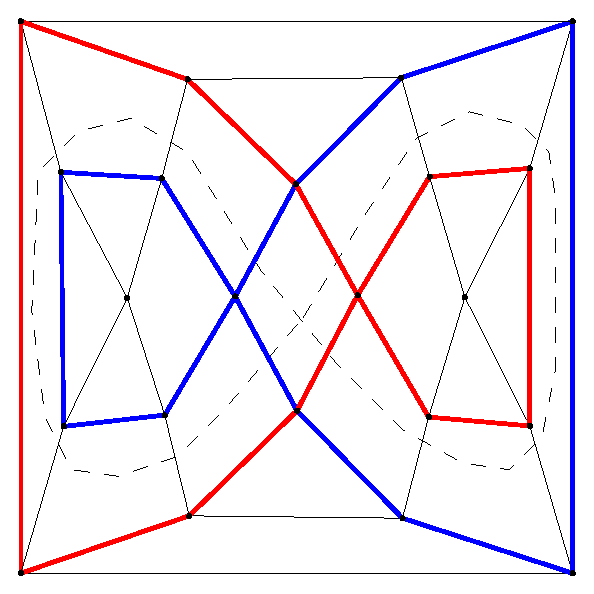
\epsfig{file=CanadaPicture/ExampleRedSelfSec.eps, height=4cm}\par
%$oc_{22}(C_{2v})$
\end{minipage}
\end{center}

Railroads, as well as central circuits, can be self-intersecting. An octahedrite is called \textcolor{red}{tight} if it has no railroad.

\end{slide}







\begin{slide}{Railroads, $3$-valent case}
A \textcolor{red}{railroad} in graph $q_n$, $q=3, 4, 5$ is a circuit of hexagonal faces, such that any of them is adjacent to its neighbors on opposite faces. Any railroad is bordered by two zigzags.

\begin{center}
\begin{minipage}{5.5cm}
\centering
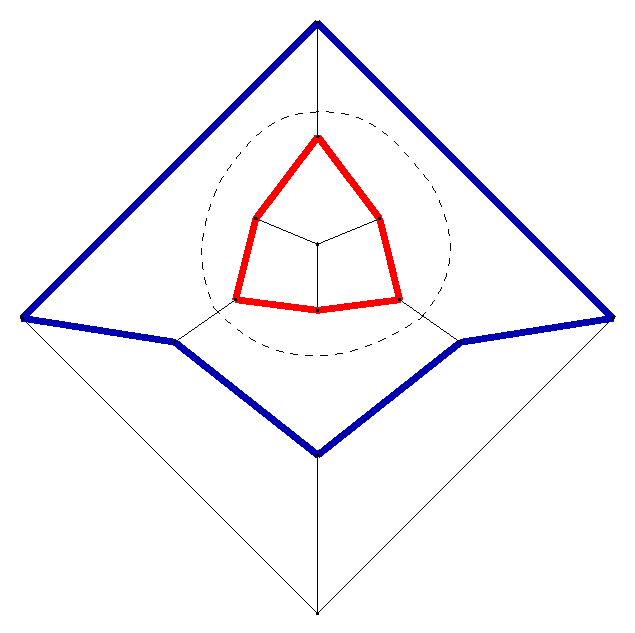
\epsfig{file=ZIGZAGpicture/Graph4n_14_1sec, height=4cm}\par
$4_{14}(D_{3h})$
\end{minipage}
\begin{minipage}{5.5cm}
\centering
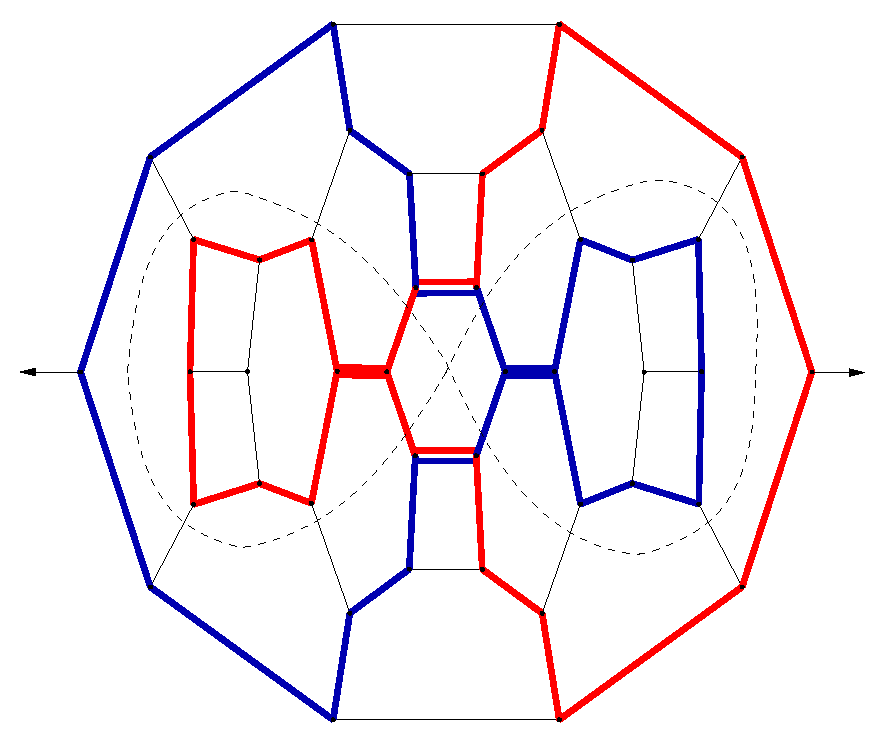
\epsfig{file=ZIGZAGpicture/Graph42_54th.eps, height=4cm}\par
$4_{42}(C_{2v})$
\end{minipage}
\end{center}

Railroads, as well as zigzags, can be self-intersecting (\textcolor{red}{doubly} or \textcolor{red}{triply}). A graph $q_n$ is called \textcolor{red}{tight} if it has no railroad.



\end{slide}





\begin{slide}{Triple self-intersection}

\begin{center}
\begin{minipage}{5.5cm}
\centering
\epsfig{file=ZIGZAGpicture/ZZint111Railroad066_11-color.eps, height=5cm}\par
$4_{66}(D_{3h})$\\
It is smallest such $4_n$ graph.
\end{minipage}
\begin{minipage}{5.5cm}
\centering
\epsfig{file=ZIGZAGpicture/DutourFull4th-color.eps,height=5cm}\par
$5_{176}(C_{3v})$\\
\textcolor{red}{Conjecture:} It is smallest such $5_n$ graph.
\end{minipage}

\end{center}
\end{slide}






\overlays{3}{
\begin{slide}{Removing central circuits}
\onlySlide*{1}{\centering
Take a $4$-valent plane graph $G$ and a central circuit.\par
\resizebox{80mm}{!}{\rotatebox{0}{\includegraphics{CanadaPicture/GraphRemoveCCstep1.eps}}}\par
}%
\onlySlide*{2}{\centering
Remove the edges of the central circuit.\par
\resizebox{80mm}{!}{\rotatebox{0}{\includegraphics{CanadaPicture/GraphRemoveCCstep2.eps}}}\par
}%
\onlySlide*{3}{\centering
Remove the vertices of degree $0$ or $2$.\par
\resizebox{80mm}{!}{\rotatebox{0}{\includegraphics{CanadaPicture/GraphRemoveCCstep3.eps}}}\par
}%
\end{slide}
}


\overlays{4}{
\begin{slide}{Removing zigzags}
%\onlySlide*{1}{\centering
%Take a plane graph $G$ and a zigzag\par
%\resizebox{80mm}{!}{\rotatebox{0}{\includegraphics{PL_D6_7sec.eps}}}\par
%}%
\onlySlide*{1}{\centering
Take a plane graph $G$ and a zigzag.\par
\resizebox{80mm}{!}{\rotatebox{0}{\includegraphics{CanadaPicture/PL_D6_7thi.eps}}}\par
}%
\onlySlide*{2}{\centering
Go to the medial.\par
\resizebox{80mm}{!}{\rotatebox{0}{\includegraphics{CanadaPicture/GraphMedPL_D6_7sec.eps}}}\par
}%
\onlySlide*{3}{\centering
Remove the central circuit.\par
\resizebox{80mm}{!}{\rotatebox{0}{\includegraphics{CanadaPicture/GraphMedPL_D6_7thi.eps}}}\par
}%
\onlySlide*{4}{\centering
Take one (out of two) inverse medial graph.
\resizebox{80mm}{!}{\rotatebox{0}{\includegraphics{CanadaPicture/PL_D6_7der2_5.ps}}}\par
}%

\end{slide}
}





\begin{slide}{Extremal problem}
Given a class of tight graphs (octahedrites, graphs $q_n$), there exist a constant \textcolor{red}{$C$} such that any element of the class has at most \textcolor{red}{$C$} ZC-circuits.

\begin{itemize}
\item Every tight octahedrite has at most \textcolor{red}{$6$} central circuits.\\
\textcolor{red}{Proof method:} Local analysis + case by case analysis.
\item Every tight $3_n$ has exactly \textcolor{red}{$3$} zigzags.\\
\textcolor{red}{Proof method:} Uses an algebraic formalism on the graphs $3_n$.
\item Every tight $4_n$ has at most \textcolor{red}{$9$} zigzags.\\
\textcolor{red}{Conjecture:} The correct upper bound is $8$. Checked for $n\leq 400$.
\item Every tight $5_n$ has at most \textcolor{red}{$15$} zigzags.\\
\textcolor{red}{Attempted proof:} Uses a local analysis on zigzags.

\end{itemize}



\end{slide}









\overlays{2}{
\begin{slide}{Tight with simple central circuits}
\fromSlide{1}{
\begin{theorem}
There is exactly \textcolor{red}{$8$} tight octahedrites with simple central circuits.\\
\end{theorem}
\textcolor{red}{Proof method:} After removing a central circuit, the obtained graph has faces of gonality at most $4$.\\
}%
\onlySlide*{1}{\small
\setlength{\unitlength}{1cm}
\begin{minipage}{2.8cm}
\centering
\epsfig{file=CanadaPicture/OctahedronCCsec.eps, width=28mm}\par
{\bf 6} \quad $O_h$\\
$4^3$
\end{minipage}
\begin{minipage}{2.8cm}
\centering
\epsfig{file=CanadaPicture/CuboctahedronCCsec.eps, width=28mm}\par
{\bf 12} \quad $O_h$\\
$6^4$
\end{minipage}
\begin{minipage}{2.8cm}
\centering
\epsfig{file=CanadaPicture/8-hedrite12-1sec.eps, width=28mm}\par
{\bf 12} \quad $D_{3h}$\\
$6^4$
\end{minipage}
\begin{minipage}{2.8cm}
\centering
\epsfig{file=CanadaPicture/SimpleCC14sec.eps, width=28mm}\par
{\bf 14} \quad $D_{4h}$\\
$6^2,8^2$
\end{minipage}
}%
\onlySlide*{2}{\small
\begin{minipage}{2.8cm}
\centering
\epsfig{file=CanadaPicture/PureOctahedrite20.eps, width=28mm}\par
{\bf 20} \quad $D_{2d}$\\
$8^5$
\end{minipage}
% \setlength{\unitlength}{1cm}
\begin{minipage}{2.8cm}
\centering
\epsfig{file=CanadaPicture/PureOctahedrite22.eps, width=28mm}\par
{\bf 22} \quad $D_{2h}$\\
$8^3,10^2$
\end{minipage}
\begin{minipage}{2.8cm}
\centering
\epsfig{file=CanadaPicture/oc30-1thi.eps, width=28mm}\par
{\bf 30} \quad $O$\\
$10^6$
\end{minipage}
\begin{minipage}{2.8cm}
\centering
\epsfig{file=CanadaPicture/PureOctahedrite32-1.eps, width=28mm}\par
{\bf 32} \quad $D_{4h}$\\
$10^4,12^2$
\end{minipage}
}%
\end{slide}
}








\begin{slide}{Tight with simple zigzags}

\begin{itemize}
\item All tight $3_n$ have simple zigzags\\
\ding{224}\textcolor{red}{Infinity} of such graphs
\item There are exactly \textcolor{red}{$2$} tight graph $4_n$ with simple zigzags: Cube and Truncated Octahedron=$GC_{1,1}(Cube)$.\\
\begin{minipage}{5.0cm}
\textcolor{red}{Proof method:} The size of intersection of two simple zigzags is at most $6$. There is at most $9$ zigzags.\\
\ding{224}\textcolor{red}{Upper bound} on $n$.
\end{minipage}
\begin{minipage}{5.2cm}
\begin{minipage}{2.5cm}
\centering
\epsfig{file=CanadaPicture/ExamplSimple4n.eps, height=18mm}\par
{\bf 6} \quad $O_h$, $6^4$
\end{minipage}
\begin{minipage}{2.5cm}
\centering
\epsfig{file=CanadaPicture/TrOctahedronSec.eps, height=18mm}\par
{\bf 24} \quad $O_{h}$, $10^6$
\end{minipage}
\end{minipage}

\item There is at least \textcolor{red}{$9$} tight graphs $5_n$ with simple zigzags.\\
\textcolor{blue}{G. Brinkmann and T. Harmuth} computation of fullerenes with simple zigzags up to $200$ vertices.
\end{itemize}

\end{slide}




\overlays{2}{
\begin{slide}{Tight $5_n$ with simple zigzags}
\onlySlide*{1}{
\vspace{-5mm}
\begin{minipage}[b]{3.7cm}
\centering
\resizebox{32mm}{!}{\includegraphics{CanadaPicture/Tight20_Ihsec.eps}}\par
$20$ \quad $I_h$, $20^6$
\end{minipage}
\begin{minipage}[b]{3.7cm}
\centering
\resizebox{37mm}{!}{\includegraphics{CanadaPicture/Tight28_Tdsec.eps}}\par
$28$ \quad $T_d$, $12^7$
\end{minipage}
\begin{minipage}[b]{3.7cm}
\centering
\resizebox{37mm}{!}{\includegraphics{CanadaPicture/Tight48_D3sec1.eps}}\par
$48$ \quad $D_3$, $16^9$
\end{minipage}
\begin{minipage}[b]{3.7cm}
\centering
\resizebox{37mm}{!}{\includegraphics{CanadaPicture/Tight60_D3sec.eps}}\par
$60$ \quad $D_3$, $18^{10}$
\end{minipage}
\begin{minipage}[b]{3.7cm}
\centering
%\resizebox{37mm}{!}{\includegraphics{Tight60_Ihsec.eps}}\par
\resizebox{37mm}{!}{\includegraphics{CanadaPicture/TightIhSimple.eps}}\par
$60$ \quad $I_h$, $18^{10}$
\end{minipage}
\begin{minipage}[b]{3.7cm}
\centering
\resizebox{37mm}{!}{\includegraphics{CanadaPicture/Tight76_D2dsec1.eps}}\par
$76$ \quad $D_{2d}$, $22^4, 20^7$
\end{minipage}
}%
\onlySlide*{2}{
\begin{minipage}[b]{3.7cm}
\centering
\resizebox{37mm}{!}{\includegraphics{CanadaPicture/Tight88_Tsec.eps}}\par
$88$ \quad $T$, $22^{12}$
\end{minipage}
\hfill\begin{minipage}[b]{3.7cm}
\centering
\resizebox{37mm}{!}{\includegraphics{CanadaPicture/Tight92_Thsec.eps}}\par
$92$ \quad $T_h$, $24^6, 22^6$
\end{minipage}
\begin{center}
\vspace{-2cm}
\begin{minipage}[b]{5cm}
\centering
\resizebox{43mm}{!}{\includegraphics{CanadaPicture/Tight140_Isec.eps}}\par
$140$ \quad $I$, $28^{15}$
\end{minipage}
\end{center}
}%
\end{slide}
}






%\begin{slide}{Tight $5_n$ with only simple zigzags}
%{\scriptsize
%\begin{center}
%\begin{tabular}{||c|c|l|l|c||}
%\hline
%\hline
%$n$       &group          &$z$-vector     &orbit lengths  &int. vector\\
%\hline \hline
%$20$    &$I_h$          &$10^6$         &6              &$2^5$ \\
%$28$    &$T_d$          &$12^7$         &3,4            &$2^6$\\
%$48$    &$D_3$          &$16^9$         &3,3,3          &$2^8$\\
%$60$    &$I_h$          &$18^{10}$      &10             &$2^9$\\
%$60$    &$D_3$          &$18^{10}$      &1,3,6          &$2^9$\\
%$76$    &$D_{2d}$       &$22^4,20^7$    &1,2,4,4        &$4,2^9$ and $2^{10}$\\
%$88$    &$T$            &$22^{12}$      &12             &$2^{11}$\\
%$92$    &$T_h$          &$22^6, 24^6$   &6,6            &$2^{11}$ and $2^{10}, 4$\\
%$140$   &$I$            &$28^{15}$      &15             &$2^{14}$\\
%\hline
%\hline
%\end{tabular}
%\end{center}
%}
%Conjecture: this list is complete (checked for $n\leq 200$).

%It gives $7$ \textcolor{red}{Gr\"unbaum arrangements} of plane curves.
%
%\end{slide}






%%%%%%%%%%%%%%%%%%%% Slide presentation
\begin{slide}{}
\begin{center}
{\Huge 
\begin{tabular*}{8cm}{c}
\\[-0.5cm]
\textcolor{blue}{IV. }\textcolor{red}{Goldberg-Coxeter}\\
\textcolor{red}{construction}
\end{tabular*}
}
\end{center}
\end{slide}

%%%%%%%%%%%%%%%%%%%%  the construction
\begin{slide}{The construction}
\begin{itemize}
\item Take a $3$- or $4$-valent plane graph $G_0$. The graph $G_0^{*}$ is formed of triangles or squares.
\item Break the triangles or squares into pieces according to parameter $(k,l)$.
\end{itemize}
\begin{center}
\epsfig{file=GOLDBERGpicture/GoldbergBreakdown.eps,width=105mm}
\end{center}

\end{slide}


%%%%%%%%%%%%%%%%%%% sequel of construction
%\overlays{4}{
\begin{slide}{Gluing the pieces}
%\fromSlide{1}{
\begin{itemize}
\item Glue the pieces together in a coherent way.
\item We obtain another \textcolor{red}{triangulation} or \textcolor{red}{quadrangulation} of the plane.
\end{itemize}
%}%
%\onlySlide*{1}{
%\begin{center}
%\begin{minipage}{5.5cm}
%\centering
%\epsfig{file=SimpleCaseOfConstruction3-valent1.eps,width=48mm}\par
%Case $3$-valent
%\end{minipage}
%\begin{minipage}{5.5cm}
%\centering
%\epsfig{file=SimpleCaseOfConstruction4-valent1.eps,width=48mm}\par
%Case $4$-valent
%\end{minipage}
%\end{center}
%}%
%\onlySlide*{2}{
%\begin{center}
%\begin{minipage}{5.5cm}
%\centering
%\epsfig{file=SimpleCaseOfConstruction3-valent2.eps,width=48mm}\par
%$(3,0)$: $3$-valent
%\end{minipage}
%\begin{minipage}{5.5cm}
%\centering
%\epsfig{file=SimpleCaseOfConstruction4-valent2.eps,width=48mm}\par
%$(3,0)$: $4$-valent
%\end{minipage}
%\end{center}
%}%
%\onlySlide*{3}{
%\begin{center}
%\centering
%\epsfig{file=GOLDBERGpicture/MergingBreakdown1.eps,width=50mm}
%\end{center}
%}%
%\onlySlide*{4}{
\begin{center}
\centering
\epsfig{file=GOLDBERGpicture/MergingBreakdown2.eps,width=50mm}
\end{center}
%}%
\end{slide}
%}








\begin{slide}{Final steps}

\begin{itemize}
\item Go to the dual and obtain a $3$- or $4$-valent plane graph, which is denoted $GC_{k,l}(G_0)$ and called ``\textcolor{red}{Goldberg-Coxeter construction}''.
\item The construction works for any $3$- or $4$-valent map on \textcolor{red}{oriented surface}.
\end{itemize}
\vspace{-2mm}
\begin{center}
\begin{minipage}[t]{7cm}
\centering
\epsfxsize=6cm
\epsffile{GOLDBERGpicture/eberhardSec.eps}\par
\end{minipage}
\begin{minipage}[t]{3cm}
\centering
\epsfxsize=2.7cm
\epsffile{GOLDBERGpicture/C80Sec.eps}\par
\end{minipage}
\end{center}
\begin{center}
Operation $GC_{2,0}$ on Tetrahedron, Cube and Dodecahedron
\end{center}




\end{slide}









%%%%%%%%%%%% an example at length.

%\overlays{7}{
%\begin{slide}{Example of $GC_{3,2}(Octahedron)$}
%%\onlySlide*{1}{\begin{center}\epsfig{file=Octahedron.eps,width=80mm}\end{center}}%
%\onlySlide*{1}{\begin{center}\epsfig{file=OctahedronSec.eps,width=100mm}\end{center}}%
%%\onlySlide*{2}{\begin{center}\epsfig{file=dualPL32sec.eps,width=80mm}\end{center}}%
%\onlySlide*{2}{\begin{center}\epsfig{file=NewDualPL32secNr1.eps,width=107mm}\end{center}}%
%\onlySlide*{3}{\begin{center}\epsfig{file=NewDualPL32secNr1_2.eps,width=107mm}\end{center}}%
%\onlySlide*{4}{\begin{center}\epsfig{file=NewDualPL32secNr2.eps,width=107mm}\end{center}}%
%\onlySlide*{5}{\begin{center}\epsfig{file=NewDualPL32secNr3.eps,width=107mm}\end{center}}%
%\onlySlide*{6}{\begin{center}\epsfig{file=NewDualPL32secNr4.eps,width=107mm}\end{center}}%
%%\onlySlide*{3}{\begin{center}\epsfig{file=dualPL32secSquares.eps,width=80mm}\end{center}}%
%%\onlySlide*{6}{\begin{center}\epsfig{file=nPL32thi.eps,width=80mm}\end{center}}%
%\onlySlide*{7}{\begin{center}\epsfig{file=3foldViewPL32sec.eps,width=70mm}\end{center}}%
%\end{slide}
%}




\begin{slide}{Goldberg-Coxeter for Cube}
\vspace{-5mm}
\begin{center}
\begin{minipage}{4.0cm}
\centering
\epsfig{file=GOLDBERGpicture/Cube1_0-sec.eps,width=35mm}
\end{minipage}
\begin{minipage}{4.0cm}
\centering
\epsfig{file=GOLDBERGpicture/Cube1_1-sec.eps,width=35mm}
\end{minipage}
\begin{minipage}{4.0cm}
\centering
\epsfig{file=GOLDBERGpicture/Cube2_0-sec.eps,width=35mm}
\end{minipage}
\begin{minipage}{4.0cm}
\centering
\epsfig{file=GOLDBERGpicture/Cube2_1-sec.eps,width=35mm}
\end{minipage}
\end{center}
\end{slide}



\begin{slide}{Goldberg-Coxeter for Octahedron}
\vspace{-4mm}
\begin{center}
\begin{minipage}{4.0cm}
\centering
\epsfig{file=GOLDBERGpicture/Octahedron1_0sec.eps,width=30mm}
\end{minipage}
\begin{minipage}{4.0cm}
\centering
\epsfig{file=GOLDBERGpicture/Octahedron1_1sec.eps,width=30mm}
\end{minipage}
\begin{minipage}{4.0cm}
\centering
\epsfig{file=GOLDBERGpicture/Octahedron2_0sec.eps,width=30mm}
\end{minipage}
\begin{minipage}{4.0cm}
\centering
\epsfig{file=GOLDBERGpicture/Octahedron2_1sec.eps,width=30mm}
\end{minipage}
\end{center}
\end{slide}








\begin{slide}{Properties}
\vspace{-3mm}
\begin{itemize}
\item One associates \textcolor{red}{$z=k+le^{i\frac{\pi}{3}}$(Eisenstein integer)} or \textcolor{red}{$z=k+li$(Gaussian integer)} to the pair $(k,l)$ in $3$- or $4$-valent case.

\item If one writes \textcolor{red}{$GC_{z}(G_0)$} instead of $GC_{k,l}(G_0)$, then one has:
\begin{equation*}
\begin{array}{rcl}
\textcolor{blue}{GC_{z}(GC_{z'}(G_0))}  &=&\textcolor{blue}{GC_{zz'}(G_0)}
%GC_{\overline{z}}(G_0)&=&GC_{z}(\overline{G_0})
\end{array}
\end{equation*}
%with $\overline{G_0}$ the symmetric on a plane of $G_0$.

%\item[\ding{108}] $GC_{1,0}(G_0)=G_0$
\item If $G_0$ has $n$ vertices, then $GC_{k,l}(G_0)$ has 
\begin{center}
\begin{tabular}{rcl}
$n(k^2+kl+l^2)=n|z|^2$ vertices &if& $G_0$ is \textcolor{red}{$3$-valent},\\
$n(k^2+l^2)=n|z|^2$ vertices &if& $G_0$ is \textcolor{red}{$4$-valent}.
\end{tabular}
\end{center}
\item If $G_0$ has a symmetry plane, then \textcolor{blue}{$GC_{z}(G_0)=GC_{\overline{z}}(G_0)$}.
\item $GC_{z}(G_0)$ has all \textcolor{red}{rotational symmetries} of $G_0$ and all symmetries if $l=0$ or $l=k$.
\end{itemize}

\end{slide}



%%%%%%%%%%% medial and leapfrog
%\overlays{3}{
%\begin{slide}{The case $(k,l)=(1,1)$}
%\onlySlide*{1}{
%\begin{center}
%\begin{minipage}{5.5cm}
%\centering
%\epsfig{file=ExampleLeapFrog1.eps,width=50mm}\par
%Case $3$-valent
%\end{minipage}
%\begin{minipage}{5.5cm}
%\centering
%\epsfig{file=ExampleMedial1.eps,width=50mm}\par
%\vspace{0.9cm}
%Case $4$-valent
%\end{minipage}
%\end{center}
%}
%\onlySlide*{2}{
%\begin{center}
%\begin{minipage}{5.5cm}
%\centering
%\epsfig{file=ExampleLeapFrog2.eps,width=50mm}\par
%Case $3$-valent
%\end{minipage}
%\begin{minipage}{5.5cm}
%\centering
%\epsfig{file=ExampleMedial2.eps,width=50mm}\par
%\vspace{0.9cm}
%Case $4$-valent
%\end{minipage}
%\end{center}
%}
%\onlySlide*{3}{
%\begin{center}
%\begin{minipage}{5.5cm}
%\centering
%\epsfig{file=ExampleLeapFrog3.eps,width=50mm}\par
%Case $3$-valent\par
%$GC_{1,1}$ is called \textcolor{red}{leapfrog}
%(=Truncation of the dual)
%\end{minipage}
%\begin{minipage}{5.5cm}
%\centering
%\epsfig{file=ExampleMedial3.eps,width=50mm}\par
%\vspace{0.9cm}
%Case $4$-valent\par
%$GC_{1,1}$ is called \textcolor{red}{medial}\par
%\textcolor{white}{Bonjour}
%\end{minipage}
%\end{center}
%}
%\end{slide}
%}


%%%%%%%%%%%%%%   Goldberg Theorem's
%\begin{slide}{Goldberg Theorem}
%
%
%\begin{center}
%{\small
%\begin{tabular}{||c|c|c|c||}
%\hline
%\hline
%Class&             &Groups    &Construction\\
%\hline
%$3_n$&$p_3=4$      &$T$, $T_d$&$GC_{k,l}(\mbox{Tetrahedron})$\\
%$4_n$&$p_4=6$      &$O$, $O_h$&$GC_{k,l}(\mbox{Cube})$\\
%$4_n$&$p_4=6$      &$D_6$, $D_{6h}$&$GC_{k,l}(\mbox{Prism}_6)$\\
%$5_n$&$p_5=12$     &$I$, $I_h$&$GC_{k,l}(\mbox{Dodecahedron})$\\\hline
%Octahedrites&$p_3=8$&$O$, $O_h$&$GC_{k,l}(\mbox{Octahedron})$\\
%\hline
%\hline
%\end{tabular}
%}
%\end{center}
%\end{slide}












%%%%%%%%%%%%%%  k-inflation theorem
\overlays{3}{
\begin{slide}{The special case $GC_{k,0}$}
\fromSlide{1}{
\vspace{-2mm}
\begin{itemize}
\item Any ZC-circuit of $G_0$ corresponds to \textcolor{red}{$k$ ZC-circuits} of $GC_{k,0}(G_0)$ with length \textcolor{red}{multiplied by $k$}.
\item If the ZC-vector of $G_0$ is $\dots, c_l^{m_l}, \dots$, then the ZC-vector of $GC_{k,0}(G_0)$ is \textcolor{red}{$\dots, (kc_l)^{km_l}, \dots$}.
\end{itemize}
}
\onlySlide*{1}{
\begin{center}
\begin{minipage}{5.5cm}
\centering
\epsfig{file=GOLDBERGpicture/Cube10Sec.eps,width=50mm}
\end{minipage}
\begin{minipage}{5.5cm}
\centering
\epsfig{file=GOLDBERGpicture/Octahedron10Sec.eps,width=50mm}
\end{minipage}
\end{center}
}%
\onlySlide*{2}{
\begin{center}
\begin{minipage}{5.5cm}
\centering
\epsfig{file=GOLDBERGpicture/Cube20Sec.eps,width=50mm}
\end{minipage}
\begin{minipage}{5.5cm}
\centering
\epsfig{file=GOLDBERGpicture/Octahedron20Sec.eps,width=50mm}
\end{minipage}
\end{center}
}%
\onlySlide*{3}{
\begin{center}
\begin{minipage}{5.5cm}
\centering
\epsfig{file=GOLDBERGpicture/Cube30Sec.eps,width=50mm}
\end{minipage}
\begin{minipage}{5.5cm}
\centering
\epsfig{file=GOLDBERGpicture/Octahedron30Sec.eps,width=50mm}
\end{minipage}
\end{center}
}%

\end{slide}
}




\begin{slide}{$(k,l)$-product formalism}
Given a $3$-valent plane graph $G$, the zigzags of the Goldberg-Coxeter construction of $GC_{k,l}(G)$ are obtained by:

\begin{itemize}
\item associating to $G$ two elements $L$ and $R$ of a group called \textcolor{red}{moving group},
\item computing the value of the \textcolor{red}{$(k,l)$-product} $L\odot_{k,l} R$,
\item the lengths of zigzags are obtained by computing the \textcolor{red}{cycle structure} of $L\odot_{k,l} R$.
\end{itemize}
For $GC_{k,l}(Dodecahedron)$ with $gcd(k,l)=1$, this gives $6$, $10$ or $15$ zigzags.


%{\scriptsize
%
%M. Dutour and M. Deza, {\em Goldberg-Coxeter construction for $3$- or $4$-valent plane graphs}, Electronic Journal of Combinatorics, {\bf 11-1} (2004) R20.
%}


\end{slide}






\begin{slide}{Illustration}
\vspace{-2mm}
\begin{itemize}
\item For any ZC-circuit of $GC_{k,l}(G_0)$, there exist $\alpha\geq 1$
\begin{tabular}{lll}
${\rm length}(ZC)$=$2(k^2+kl+l^2)\alpha$& \textcolor{red}{$3$-valent case}\\
${\rm length}(ZC)$=$(k^2+l^2)\alpha$ & \textcolor{red}{$4$-valent case}
\end{tabular}

The \textcolor{red}{[ZC]-vector} of $GC_{k,l}(G_0)$ is the vector $\dots, \alpha_k^{m_k}, \dots$ where $m_k$ is the number of ZC-circuits with \textcolor{red}{order} $\alpha_k$.
\item If $gcd(k,l)=1$, then $GC_{k,l}(Cube)$ has $6$ zigzags if $k\equiv l\pmod 3$ and $4$ otherwise.
\item For \textcolor{red}{Truncated Icosidodecahedron}, possible [ZC]:
\begin{center}
\begin{minipage}{3cm}
\begin{center}
\epsfig{file=GOLDBERGpicture/TruncatedIcosidodecahedron.ps,width=30mm}
\end{center}
\end{minipage}
\begin{minipage}{6cm}
\textcolor{red}{
\begin{tabular}{|l|l|l|}
\hline
$2^{30}, 3^{40}$&
$2^{30}, 5^{24}$&
$3^{20}, 5^{24}$\\
$2^{60}, 3^{20}$&
$2^{60}, 5^{12}$&
$3^{40}, 5^{12}$\\
$2^{90}$&
$3^{60}$&
$5^{36}$\\
$9^{20}$&
$6^{30}$&
$15^{12}$\\
\hline
\end{tabular}
}
\end{minipage}
\end{center}



\end{itemize}


\end{slide}



%\begin{slide}{Iteration}
%\vspace{-3mm}
%\begin{itemize}
%\item ``Position mapping'' is denoted \textcolor{red}{$PM(\overrightarrow{e}, p)$}=\textcolor{red}{$(\overrightarrow{f}_1, \phi_{k,l}(p))$} or \textcolor{red}{$(\overrightarrow{f}_2, \phi_{k,l}(p))$}
%\item $PM^{k+l}(\overrightarrow{e}, 1)$=$(\overrightarrow{e}', 1)$. So, one defines ``Iterated position mapping'' as \textcolor{red}{$IPM(\overrightarrow{e})=\overrightarrow{e}'$}.
%\item \textcolor{red}{${\cal DE}$} is the set of directed edges of $G_0^*$. $IPM$ is a permutation of ${\cal DE}$.
%\item For every ZC-circuit with pair $(\overrightarrow{e}, 1)$ denote \textcolor{red}{$Ord(ZC)$} the smallest $s>0$, such that $IPM^s(\overrightarrow{e})=\overrightarrow{e}$.
%\item[\ding{224}] For any ZC-circuit of $GC_{k,l}(G_0)$ one has:
%\begin{tabular}{lll}
%${\rm length}(ZC)$=$2(k^2+kl+l^2)Ord(ZC)$& $3$-valent case\\
%${\rm length}(ZC)$=$(k^2+l^2)Ord(ZC)$ & $4$-valent case
%\end{tabular}
%
%The \textcolor{red}{[ZC]-vector} of $GC_{k,l}(G_0)$ is the vector $\dots, c_k^{m_k}, \dots$ where $m_k$ is the number of ZC-circuits with \textcolor{red}{order} $c_k$.

%If ZC of $GC_{k,l}(G_0)$ is \dots, $c_k^{m_k}$,\dots then \textcolor{red}{[ZC]} of $GC_{k,l}(G_0)$ is \dots, $\{\frac{c_k}{2(k^2+kl+l^2)}\}^{m_k}$,\dots or \dots, $\{\frac{c_k}{k^2+l^2}\}^{m_k}$,\dots.


%\item[\ding{108}] Denote [ZC]=
% the ZC-vector of $GC_{k,l}(G_0)$ with $c_k$ being the length divided by $2(k^2+kl+l^2)$ or $k^2+l^2$.
%\end{itemize}
%\end{slide}











%%%%%%%%%%%%%%%%%%%%  The moving group

%\begin{slide}{Moving group and Key Theorem}
%\begin{itemize}
%\item \textcolor{red}{$Mov(G_0)=\langle L, R\rangle$} is the \textcolor{red}{moving group}
%
%\textcolor{red}{In Cube}: a subgroup of $Sym(24)$.
%
%\item For $u\in Mov(G_0)$, denote \textcolor{red}{$ZC(u)$} the vector $\dots, c_k^{m_k},\dots$ with multiplicities $m_k$ being the \textcolor{red}{half of the number of cycles of length $c_k$} in the permutation $u$ acting on the set ${\cal DE}$.
%
%\textcolor{red}{In Cube}: \textcolor{blue}{$ZC(L)=ZC(R)=3^{4}$}
%
%\item[\ding{224}] \textcolor{red}{Key Theorem} One has for all $3$- or $4$-valent plane graphs $G_0$ and all $k,l\geq 0$
%
%\begin{center}
%\textcolor{blue}{$[ZC]-vector\mbox{~of~}GC_{k,l}(G_0)= ZC(L\odot_{k,l} R)$}
%\end{center}
%
%\end{itemize}
%\end{slide}


















%%%%%%%%%%%%%%%%   the problems
%\begin{slide}{The two problems}
%
%\begin{enumerate}
%\item[\ding{224}] Compute the set of all possible [ZC] for $GC_{k,l}(G_0)$
%\begin{center}
%\begin{tabular}{p{8cm}}
%Solvable in finite time for a given $G_0$
%\end{tabular}
%\end{center}
%\vspace{1cm}
%
%\item[\ding{224}] Compute [ZC] in terms of the pair $(k,l)$
%\begin{center}
%\begin{tabular}{p{8cm}}
%Solvable in some cases.\\
%There is a subgroup $Stab(G_0)$ of $SL_2(\ZZ)$ leaving invariant the [ZC] vector
%\end{tabular}
%\end{center}
%\end{enumerate}
%\end{slide}


%%%%%%%%%%%%%%   the solution of the first problem

%\begin{slide}{Possible [ZC]-vectors}
%\begin{itemize}
%\item Denote \textcolor{red}{${\cal P}(G_0)$} the set of all pairs $(g_1,g_2)$ with $g_i\in Mov(G_0)$.
%\item Denote \textcolor{red}{$U_{L,R}$} the smallest subset of ${\cal P}(G_0)$, which contains the pair $(L,R)$ and is stable by the two operations
%\begin{equation*}
%(x,y)\mapsto (x,yx)\mbox{~~~and~~~}(x,y)\mapsto (yx,y)
%\end{equation*}
%\item[\ding{224}] \textcolor{blue}{Theorem:} The set of possible [ZC]-vectors of $GC_{k,l}(G_0)$ is equal to the set of all vectors $ZC(v)$, $ZC(w)$ with $(v,w)\in U_{L,R}$.
%\item Computable in \textcolor{red}{finite time} for a given $G_0$.
%\end{itemize}
%\end{slide}






%\begin{slide}{}
%\begin{center}
%{\Huge 
%\begin{tabular*}{7cm}{c}
%\\[0.2cm]
%\textcolor{blue}{VII. }\textcolor{red}{Parametrizing}\\[2mm]
%\textcolor{red}{graphs $q_n$}
%\end{tabular*}
%}
%\end{center}
%\end{slide}








\begin{slide}{}
\begin{center}
{\Huge 
\begin{tabular*}{7cm}{c}
\\[-0.4cm]
\textcolor{blue}{V. }\textcolor{red}{Parametrizing}\\
\textcolor{red}{graphs}
\end{tabular*}
}
\end{center}
\end{slide}











\begin{slide}{Parametrizing graphs $q_n$}
Idea: the hexagons are of zero curvature, it suffices to give relative positions of faces of non-zero curvature.
\begin{itemize}
\item \textcolor{blue}{Goldberg (1937)} All $3_n$, $4_n$ or $5_n$ of symmetry ($T$, $T_d$), ($O$, $O_h$) or ($I$, $I_h$) are given by Goldberg-Coxeter construction $GC_{k,l}$.
\item \textcolor{blue}{Fowler and al. (1988)} All $5_n$ of symmetry $D_5$, $D_6$ or $T$ are described in terms of $4$ parameters.
\item \textcolor{blue}{Graver (1999)} All $5_n$ can be encoded by $20$ integer parameters.
\item \textcolor{blue}{Thurston (1998)} The $5_n$ are parametrized by $10$ complex parameters.
\item \textcolor{blue}{Sah (1994)} Thurston's result implies that the Nrs of $3_n$, $4_n$, $5_n$ $\sim$ $n$, $n^3$, $n^9$.
\end{itemize}

\end{slide}




\begin{slide}{The structure of graphs $3_n$}

\vspace{-4mm}
\begin{center}
\begin{minipage}{5cm}
\resizebox{5cm}{!}{\includegraphics[bb=30 20 260 200, clip]{GOLDBERGpicture/Encoding3n.eps}}\par
$4$ triangles in $Z[\omega]$
\end{minipage}
\begin{minipage}{5cm}
\resizebox{5cm}{!}{\includegraphics{GOLDBERGpicture/CorrespondingGraph3n.eps}}\par
The corresponding triangulation
\end{minipage}
\end{center}

\begin{center}
\begin{minipage}{5cm}
\resizebox{3cm}{!}{\includegraphics{GOLDBERGpicture/FromTrig.ps}}\par
\end{minipage}
\begin{minipage}{5cm}
The graph $3_{20}(D_{2d})$
\end{minipage}
\end{center}

\end{slide}



\begin{slide}{$z$- and railroad-structure of graphs $3_n$}

All zigzags and railroads are simple. 
%Denote by $(Z_{i,k})_{1\leq i\leq 3, 1\leq k\leq m_i}$ the zigzags of $G$.

\begin{itemize}
\item The $z$-vector is of the form 
\begin{equation*}
\textcolor{red}{(4s_1)^{m_1}, (4s_2)^{m_2},(4s_3)^{m_3}}\mbox{~~~with~~~}\textcolor{red}{s_im_i=\frac{n}{4}};
\end{equation*}
the number of railroads is $m_1+m_2+m_3-3$.

\item $G$ has $\geq 3$ zigzags with equality if and only if it is tight.

\item If $G$ is tight, then $z(G)=n^3$ (so, each zigzag is a Hamiltonian circuit).

%(iv) $G$ is $z$-balanced and $|Z_{i,k}\cap Z_{j,l}|=\left\lbrace\begin{array}{lcl}
%0               &\mbox{~if~}    &i=j,\\
%\frac{n}{2m_im_j}     &\mbox{~if~}    &i\not= j.
%\end{array}\right.$.

\item All $3_n$ are tight if and only if $\frac{n}{4}$ is prime.

\item There exists a tight $3_n$ if and only if $\frac{n}{4}$ is odd.
\end{itemize}


\end{slide}




\begin{slide}{General theory}
\begin{center}
\textcolor{red}{Extensions}:
\end{center}
\begin{itemize}
\item $3$-valent or $4$-valent graphs.
\item Classes of graphs with fixed $p_i$, $i\not= 6$.
\item Classes with a fixed symetry.
\item Maps on surfaces.
\end{itemize}
\begin{center}
\textcolor{red}{Dictionnary}
\end{center}
\begin{center}
{\tiny
\begin{tabular}{||c|c|c||}
\hline
\hline
               &$3$-valent graph $G_0$           &$4$-valent graph $G_0$\\
\hline
ring           &Eisenstein integers $\ZZ[\omega]$ &Gaussian integers $\ZZ[i]$\\
Euler formula  &$\sum_{i} (6-i)p_i=12$           &$\sum_{i} (4-i)p_i=8$\\
zero-curvature &hexagons                         &squares\\
ZC-circuits    &zigzags                          &central circuits\\
Operation      &leapfrog graph                   &medial graph\\
\hline
\hline
\end{tabular}
}
\end{center}






\end{slide}











\begin{slide}{Number of parameters}
{\tiny
\begin{minipage}{3.7cm}
\centering
Octahedrites:\par
\begin{tabular}{||c|c||}
\hline
\hline
Group  & $\# param.$\\
\hline
\hline
$C_1$  & $6$\\
$C_2$  & $4$\\
$D_2$  & $3$\\
$D_3$  & $2$\\
$D_4$  & $2$\\
$O$    & \textcolor{red}{$1$}\\
\hline
\hline
\end{tabular}
\end{minipage}
\begin{minipage}{3.7cm}
\centering
Graphs $3_n$:\par
\begin{tabular}{||c|c||}
\hline
\hline
Groups  & $\# param.$\\
\hline
\hline
$D_2$  & $2$\\
$T$    & \textcolor{red}{$1$}\\
\hline
\hline
\end{tabular}

Graphs $4_n$:\par
\begin{tabular}{||c|c||}
\hline
\hline
Group  & $\# param.$\\
\hline
\hline
$C_1$  & $4$\\
$C_2$  & $3$\\
$D_2$  & $2$\\
$D_3$  & $2$\\
$O$    & \textcolor{red}{$1$}\\
\hline
\hline
\end{tabular}
\end{minipage}
\begin{minipage}{3.7cm}
\centering
Graph $5_n$:\par
\begin{tabular}{||c|c||}
\hline
\hline
Group  & $\# param.$\\
\hline
\hline
$C_1$  &$10$\\
$C_2$  &$6$\\
$C_3$  &$4$\\
$D_2$  &$4$\\
$D_3$  &$3$\\
$D_5$  &$2$\\
$D_6$  &$2$\\
$T$    &$2$\\
$I$    &\textcolor{red}{$1$}\\
\hline
\hline
\end{tabular}
\end{minipage}
}

If there is just one parameter, then this is Goldberg-Coxeter construction (of \textcolor{red}{Octahedron}, \textcolor{red}{Tetrahedron}, \textcolor{red}{Cube}, \textcolor{red}{Dodecahedron} for \textcolor{red}{octahedrite}, \textcolor{red}{$3_n$}, \textcolor{red}{$4_n$}, \textcolor{red}{$5_n$}, respectively).

\end{slide}


%\begin{slide}{Tightness}
%\vspace{-3mm}
%\begin{itemize}
%\item A \textcolor{red}{railroad} in a $3$-valent plane graph $G$ is a circuit of hexagons with any two of them adjacent on opposite edges.
%\begin{center}
%\begin{minipage}{4.5cm}
%\centering
%\epsfig{file=Graph4n_14_1sec.eps, height=3.5cm}\par
%\end{minipage}
%\begin{minipage}{4.5cm}
%\centering
%\epsfig{file=Railroad3nSec.eps, height=3.5cm}\par
%\end{minipage}
%\end{center}
%They are bounded by two zigzags.
%\item A graph is called \textcolor{red}{tight} if and only if it has no railroads.
%\item If a $3$- (or $4$-)valent plane graph $G_0$ has no $q$-gonal faces with $q$=$6$ (or $4$) and $gcd(k,l)=1$ then $GC_{k,l}(G_0)$ is tight.
%\end{itemize}
%\end{slide}




















\begin{slide}{Conjecture on $4_n(\textcolor{red}{D_{3h},D_{3d}\,\,or\,\, D_3})$}
\vspace{-3mm}
%D_3 is subgroup of D_3, D_{3d}, D_{3h}, D_6, D_{6h}, O, O_h
%D_{3d} is subgroup of Oh and D6h
%D_{3h} is subgroup of D6h
\begin{itemize}
\item $4_n(\textcolor{red}{D_3 \subset  D_{3h}, D_{3d}, D_6, D_{6h}, O, O_h})$ are described by two complex parameters. They exists if and only if $n\equiv 0,2\pmod 6$ and $n\geq 8$.
\begin{center}
\begin{minipage}{50mm}
\resizebox{3cm}{!}{\includegraphics{GOLDBERGpicture/KnotD3_38_4sec.eps}}\par
$4_n(\textcolor{red}{D_3})$ with one zigzag
\end{minipage}
\begin{minipage}{50mm}
\resizebox{3cm}{!}{\includegraphics{GOLDBERGpicture/KnotD3_38_4thi.eps}}\par
The defining triangles
\end{minipage}

\end{center}

%\item $4_n(\textcolor{red}{D_3 \subset  D_{3h}, D_{3d}, D_6, D_{6h}, O, O_h})$ exists if and only if $n\equiv 0,2\pmod 6$ and $n\geq 8$.\\[3mm]

\item $4_n(\textcolor{red}{D_{3d} \subset O_h, D_{6h}})$ exists if and only if $n\equiv 0,8\pmod {12}$, $n\geq 8$.

\item If $n$ increases, then part of $4_n(\textcolor{red}{D_3})$ amongst $4_n(\textcolor{red}{D_{3h},D_{3d}, D_3})$ goes to 100\%.
\end{itemize}

\end{slide}



\begin{slide}{More conjectures}
\vspace{-4mm}


\begin{itemize}
\item All $4_n$ with only simple zigzags are:
\begin{itemize}
\item $GC_{k,0}(Cube)$, $GC_{k,k}(Cube)$ and
\item the family of $4_n(\textcolor{red}{D_3\subset\dots})$ with parameters $(m,0)$ and $(i, m-2i)$ with $n=4m(2m-3i)$ and
$z=(6m-6i)^{3m-3i}, (6m)^{m-2i}, (12m-18i)^i$.
\end{itemize}
They have symmetry $\textcolor{red}{D_{3d}}$ or $\textcolor{red}{O_{h}}$ or $\textcolor{red}{D_{6h}}$
\item Any $4_n(\textcolor{red}{D_{3}\subset\dots})$ with one zigzag is a $4_n(\textcolor{red}{D_3})$.
\item For tight graphs $4_n(\textcolor{red}{D_3\subset \dots})$ the $z$-vector is of the form $a^k$ with $k\in \{1, 2, 3, 6\}$ or $a^k, b^l$ with $k,l\in \{1, 3\}$.
\item Tight $4_n(\textcolor{red}{D_{3d}})$ exist if and only if $n\equiv 0\pmod {12}$, they are z-transitive with:
\begin{itemize}
\item $z=(n/2)^6_{n/36,0}$ iff $n\equiv 24\pmod {36}$ and, otherwise,
\item $z=(3n/2)^2_{n/4,0}$ iff $n\equiv 0,12\pmod {36}$
\end{itemize}

\end{itemize}

\end{slide}
























\begin{slide}{}
\begin{center}
{\Huge 
\begin{tabular*}{5.4cm}{c}
\\[-0.5cm]
\textcolor{blue}{VI. }\textcolor{red}{Zigzags}\\
\textcolor{red}{on}\\
\textcolor{red}{surfaces}
\end{tabular*}
}
\end{center}
\end{slide}


\begin{slide}{Klein and Dyck map}
\begin{center}
\setlength{\unitlength}{1cm}
\begin{minipage}[t]{5.0cm}
\centering
\epsfig{file=ZIGZAGpicture/IIIaSec-color.eps, height=3cm}\par
Klein map: $z=8^{21}$
\end{minipage}
\hfill
\begin{minipage}[t]{4.0cm}
\centering
\epsfig{file=ZIGZAGpicture/IIIbSec-color.eps, height=3cm}\par
Dyck map: $z=6^{16}$
\end{minipage}
\end{center}

\vspace{3mm}
\begin{itemize}
\item Zigzags (and central circuits), being local notions, are defined on any surface, even on non-orientable ones.
\item Goldberg-Coxeter and parameter constructions are defined only on oriented surfaces.
\end{itemize} 

\end{slide}








\begin{slide}{Lins trialities}
\begin{tabular}{||c|c|c|c||}
\hline
$(\textcolor{red}{v},\textcolor{green}{f},\textcolor{blue}{z})\rightarrow $   &our notation          &notation in [1]  &notation in [2]\\
\hline
$(\textcolor{red}{v},\textcolor{green}{f},\textcolor{blue}{z})$               &${\cal M}$            &gem                   &${\cal M}$\\  %0
$(\textcolor{green}{f},\textcolor{red}{v},\textcolor{blue}{z})$               &${\cal M}^*$          &dual gem              &${\cal M}^*$\\  %1
$(\textcolor{blue}{z},\textcolor{green}{f},\textcolor{red}{v})$               &$phial({\cal M})$     &\textcolor{blue}{phial} gem             &$p((p({\cal M}))^*)$\\  %5
$(\textcolor{green}{f},\textcolor{blue}{z},\textcolor{red}{v})$               &$(phial({\cal M}))^*$ &skew-dual gem         &$(p({\cal M}))^*$\\  %4
$(\textcolor{red}{v},\textcolor{blue}{z},\textcolor{green}{f})$               &$skew({\cal M})$      &\textcolor{red}{skew} gem              &$p(M)$\\  %2
$(\textcolor{blue}{z},\textcolor{red}{v},\textcolor{green}{f})$               &$(skew({\cal M}))^*$  &skew-phial gem        &$p({\cal M}^*)$\\\hline  %3
\end{tabular}
Jones, Thornton (1987): those are only ``good'' dualities.
%ere are no other "good" dualities.

{\scriptsize
\begin{enumerate}
\item S. Lins, {\em Graph-Encoded Maps}, Journal Combinatorial

Theory Ser. B {\bf 32} (1982) 171--181.

\item K. Anderson and D.B. Surowski, {\em Coxeter-Petrie Complexes}

{\em of Regular Maps}, European Journal of Combinatorics {\bf 23-8} (2002) 861--880.
\end{enumerate}
}


\end{slide}



\begin{slide}{Example: Tetrahedron}
\begin{center}
\begin{minipage}{50mm}
\epsfig{file=ZIG3picture/PhialTetr.eps, height=3cm}\par
$\textcolor{blue}{phial}(Tetrahedron)$
\end{minipage}
\begin{minipage}{50mm}
\epsfig{file=ZIG3picture/SkewTetr.eps, height=3cm}\par
$\textcolor{red}{skew}(Tetrahedron)$
\end{minipage}
\end{center}
\begin{center}
Two Lins maps on projective plane.
\end{center}

\end{slide}





\begin{slide}{Bipartite skeleton case}

\begin{center}
\begin{minipage}{50mm}
\epsfig{file=ZIG3picture/SkewCube.eps, height=3cm}
\end{minipage}
\begin{minipage}{50mm}
\epsfig{file=ZIG3picture/SkewCubeBip.eps, height=3cm}
\end{minipage}
\end{center}
\begin{center}
Two representation of $\textcolor{red}{skew}(Cube)$: on Torus and as a Cube with cyclic orientation of vertices (marked by \epsfig{file=ZIGZAGpicture/Circle.eps, height=4mm}) reversed.
\end{center}
{\it 

{\bf Theorem}

For bipartite graph embedded in oriented surface, the skew operation is, in fact, reversing orientation of one of the part of the bipartition.

}




\end{slide}





%\begin{slide}{Prisms and antiprisms}
%
%Let $\chi$ denotes the Euler characteristic.
%
%{\em {\bf Conjecture}
%\begin{itemize}
%\item 
%$\textcolor{red}{skew}(Prism_m)$ has $\chi=gcd(m,4)-m$ and is oriented\\
%iff $m$ is even;
%
%\item $\textcolor{blue}{phial}(Prism_m)$ has $\chi=2+gcd(m,4)-2m$ and is non-oriented.
%
%\vspace{3mm}
%
%\item $\textcolor{red}{skew}(APrism_m)$ has $\chi=1+gcd(m,3)-2m$ and is non-oriented;
%
%
%\item $\textcolor{blue}{phial}(APrism_m)$ has $\chi=3+gcd(m,3)-2m$ and is oriented.
%\end{itemize}
%}
%
%\end{slide}







\begin{slide}{}
\vspace{-7mm}
\begin{center}
{\Large \textcolor{red}{The End}}\par
\epsfig{file=GOLDBERGpicture/ZZprojectionCube11_4sec.eps, height=6.7cm}\par
Removing $3$ central circuits of $Med(GC_{11,4}(Cube))$.
\end{center}
\end{slide}




\end{document}
